\documentclass[twoside, final, 11pt]{articleMine}
\usepackage[english]{babel} \usepackage{a4wide}
\usepackage{amsmath,amssymb,accents} \usepackage{epsfig}
\usepackage{subfigure} \usepackage{units} \usepackage{graphicx}
\usepackage[displaymath, mathlines, right]{lineno} \usepackage{xspace}
\usepackage{color} \usepackage{epic,eepic,pstricks}
\usepackage{acronym} \usepackage{wrapfig,multicol}
\usepackage{deluxetable} \usepackage{todonotes} 
\usepackage{hyperref}
\usepackage{float}
%\usepackage{slashbox}
\usepackage{lmodern} 
%\usepackage{caption}
\linenumbers
%\usepackage{showlabels}
\usepackage[draft]{showkeys}

%\usepackage[nolists, tablesfirst]{endfloat}
\graphicspath{{plots/}}
\newcommand*\patchAmsMathEnvironmentForLineno[1]{%
  \expandafter\let\csname old#1\expandafter\endcsname\csname #1\endcsname
  \expandafter\let\csname oldend#1\expandafter\endcsname\csname end#1\endcsname
  \renewenvironment{#1}%
     {\linenomath\csname old#1\endcsname}%
     {\csname oldend#1\endcsname\endlinenomath}}%
\newcommand*\patchBothAmsMathEnvironmentsForLineno[1]{%
  \patchAmsMathEnvironmentForLineno{#1}%
  \patchAmsMathEnvironmentForLineno{#1*}}%
\AtBeginDocument{%
\patchBothAmsMathEnvironmentsForLineno{equation}%
\patchBothAmsMathEnvironmentsForLineno{align}%
\patchBothAmsMathEnvironmentsForLineno{flalign}%
\patchBothAmsMathEnvironmentsForLineno{alignat}%
\patchBothAmsMathEnvironmentsForLineno{gather}%
\patchBothAmsMathEnvironmentsForLineno{multline}%
}
%\AtBeginFigures{\cleardoublepage}
%%%%%\parindent 5pt  
\parskip 1.2pt           % sets spacing between paragraphs
\def\Offline{\mbox{$\overline{\rm
Off}$\hspace{.05em}\raisebox{.4ex}{$\underline{\rm line}$}}\xspace}
\def\OfflineB{\mbox{$\bf\overline{\rm\bf
Off}$\hspace{.05em}\raisebox{.4ex}{$\bf\underline{\rm\bf line}$}}\xspace}

\def\eq#1{\begin{equation}#1\end{equation}}
%\def\al#1{\begin{align}#1\end{align}}
%\def\vc#1{{\bf #1}}
\def\pt#1{\accentset{\rightharpoonup}{#1}}
\include{myabbr}

\newcommand{\HRule}{\rule{\linewidth}{0.5mm}}
\newcommand{\VEM}{\mbox{VEM}}
\newcommand{\m}{\mbox{m}}

\let\stdsection\section  
%\renewcommand\section{\newpage\stdsection}  
 
\begin{document}

%\setpagewiselinenumbers
\modulolinenumbers[2]

%\linenumbers


\renewcommand\linenumberfont{\small\rmfamily}
\begin{center}
  \vspace*{-13ex}

  \rule{\linewidth}{0.1mm}  \\[17mm] {\huge  System  noise temperature
    measurement of EASIER/GIGADuck detectors}
     \begin{flushright}
       \small 
     
     \end{flushright}

  % 
\end{center}
% 
\vspace*{2ex} 
%
\thispagestyle{empty}
\noindent
\begin{abstract}
  \noindent
  The  system noise  temperature is  a key  characteristic of  a radio
  detector such  as EASIER's or GIGADuck's, since  it directly relates
  to the sensitivity.  Previous measurement of this characteristic for
  these antennas  were done  in laboratory by  the CROME group  and in
  situ  by  MIDAS  group.   We  present a  measurement  of  the  noise
  temperature performed  in situ for the GIGADuck  detectors using the
  Sun's microwave flux  as a calibration source.  The  sun's signal in
  the  EASIER  detectors  being  too  small, we  set  up  a  dedicated
  measurement.   We present  in this  note the  methods to  select and
  correct the monitoring data for  GIGADuck and the method to retrieve
  the  temperature  for  EASIER.    We  also  detail  the  uncertainty
  calculation to finally obtain a  noise temperature of $T_{sys} = ???
  \pm $ for GIGADuck and $T_{sys} = ???  \pm $ for EASIER.
\end{abstract}

%
\thispagestyle{empty}
%$\;$
%\listoftodos
\noindent

\newpage

\section{Expected signal}
We present in this section the calculation of the expected signal. The
main ingredients are:
\begin{itemize}
\item the sun flux (the sun flux varies with time)
\item the sun path with respect to the antenna depending on the time of the year
\item the antenna pattern
\end{itemize}
Given these  ingredients can then  calculate the expected  increase of
power collected output by the antenna and deduce the expected increase
of the baseline for a given system temperature.

\subsection{Sun flux}
In our frequency range ~ GHz,  the sun flux has two main contributions
~\cite{solarflux}:  a quiet  sun component  (or  background component)
with a constant intensity and a frequency dependence as:
\begin{equation} 
 Sq \  [SFU] =  26.4 +  12.4 \ \nu  + 1.11\  \nu^2 \\ \rm  for \  (1 <
 \nu(GHz) < 20)
\end{equation}
a    second    contribution,   the    so    called   slowly    varying
component, its spectrum is parameterised as:
\begin{equation}
    Sv  \ [SFU]= \frac{0.64 ( F10.7 - 70 ) f^{0.4}}{ 1 + 1.56 ( ln \ ( \ f  \ / \  2.9 ) )^2}
\end{equation}
These spectra are shown in the figure~\ref{fig:spectra}
\begin{figure}[!ht]
  \centering
  \hspace*{-3ex}
  \subfigure{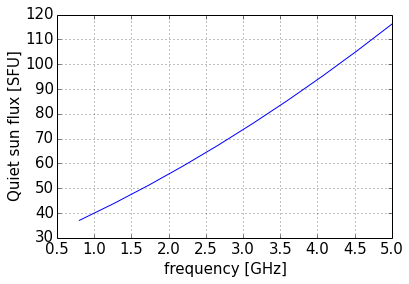
\includegraphics[width=0.49\linewidth]{quietsunspec.png}}
  \subfigure{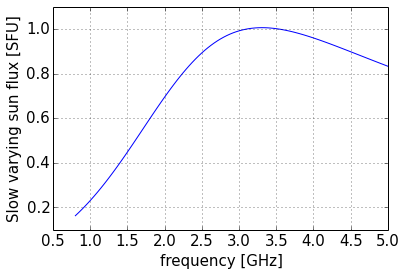
\includegraphics[width=0.49\linewidth]{varyingsunspec.png}}
  \caption{Left: quiet sun spectrum, Right: varying component spectrum}
  \label{fig:spectra}
\end{figure}
The  intensity of  the total  flux at  2.8GHz (F10.7)  is  measured by
several  observatories\cite{nobeyamaobs}, \cite{nasa}.  Making  use of
these data  and the parameterization  in frequency written  above, one
can deduce the flux in the C-band.


\paragraph{F10.7}
\begin{figure}[!ht]
  \centering
  \hspace*{-3ex}
  \subfigure{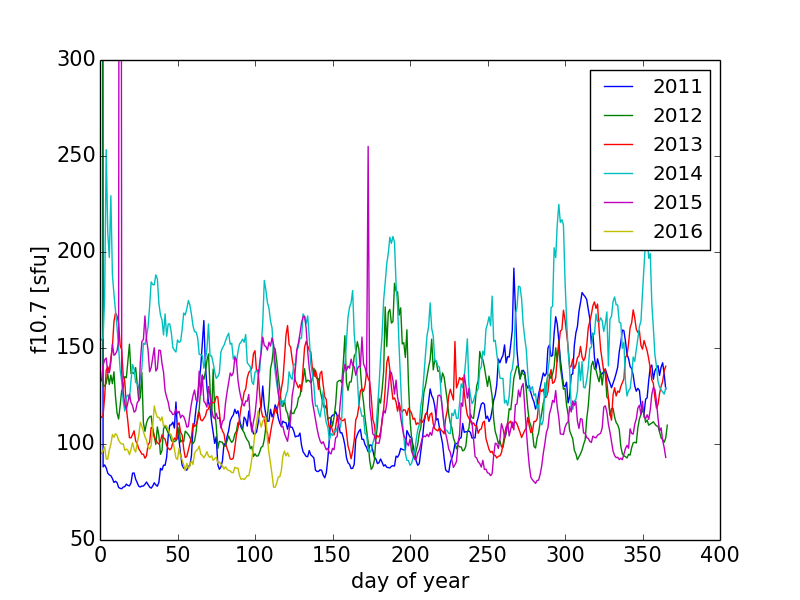
\includegraphics[width=0.7\linewidth]{f10_72011_2016.png}}
  \caption{Left: quiet sun spectrum, Right: varying component spectrum}
  \label{fig:spectra}
\end{figure}


\paragraph{sun path}
\begin{figure}[!ht]
  \centering
  \hspace*{-3ex}
  \subfigure{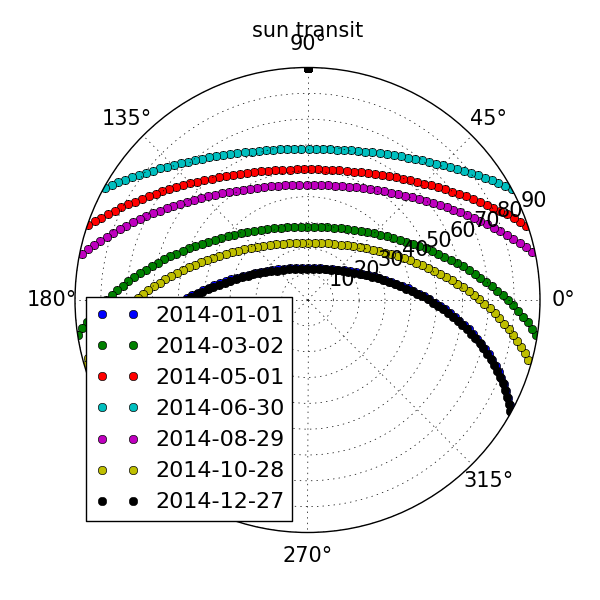
\includegraphics[width=0.7\linewidth]{sunpath.png}}
  \caption{Left: quiet sun spectrum, Right: varying component spectrum}
  \label{fig:spectra}
\end{figure}

\paragraph{expected signal}
\begin{figure}[!ht]
  \centering
  \hspace*{-3ex}
  \subfigure{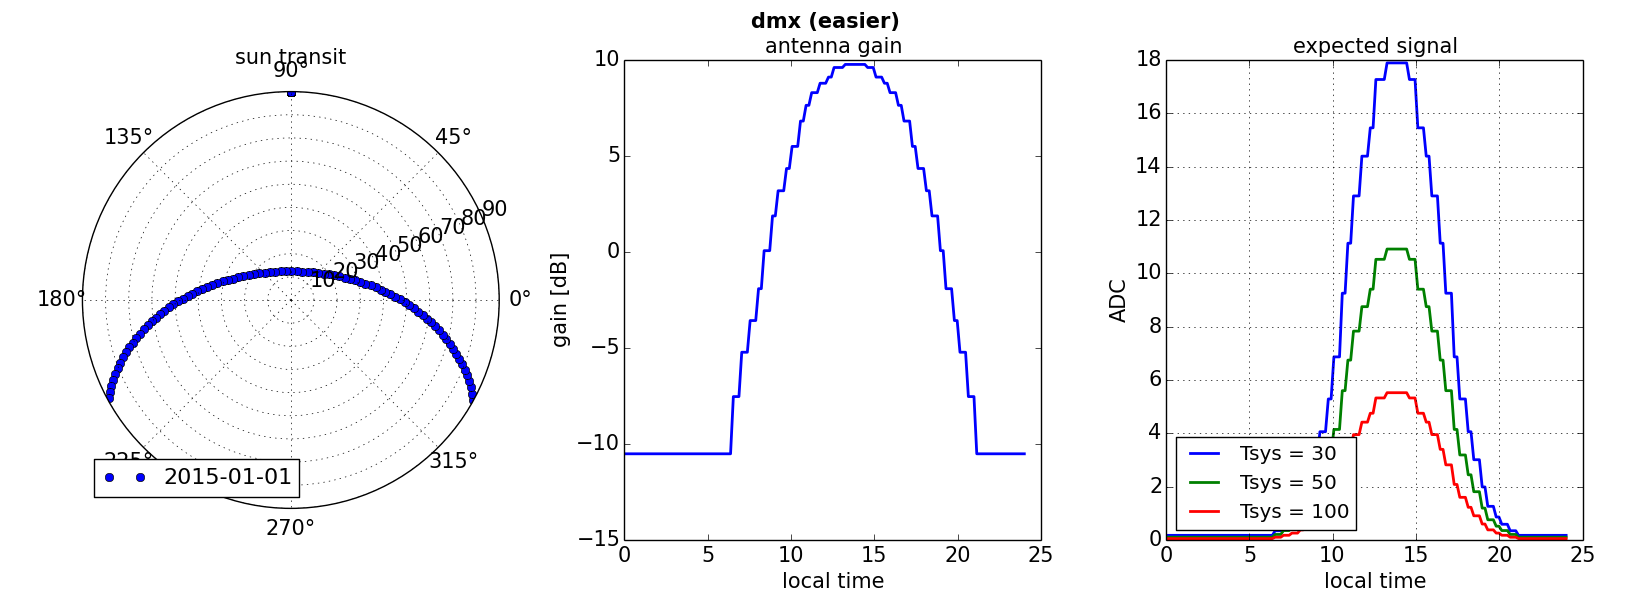
\includegraphics[width=0.7\linewidth]{expeasier.png}}\\
  \subfigure{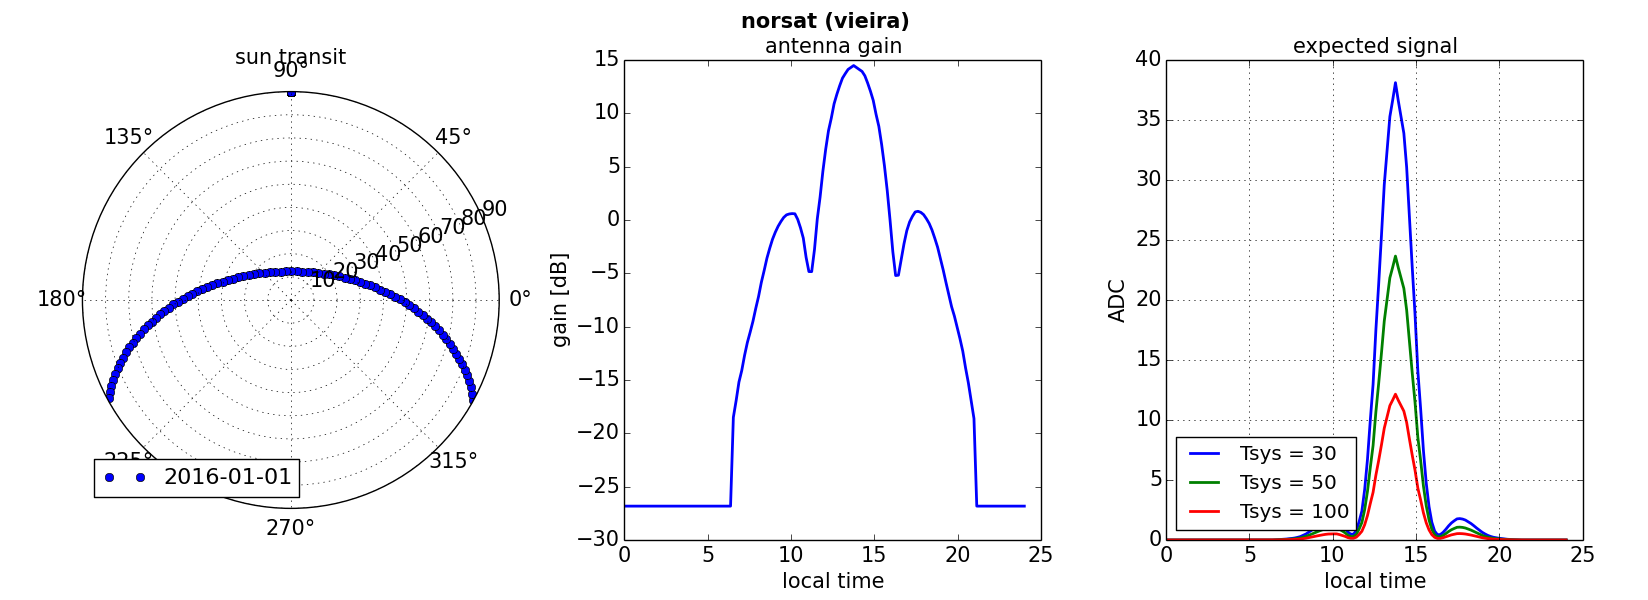
\includegraphics[width=0.7\linewidth]{expvieira20160101.png}}\\
  \subfigure{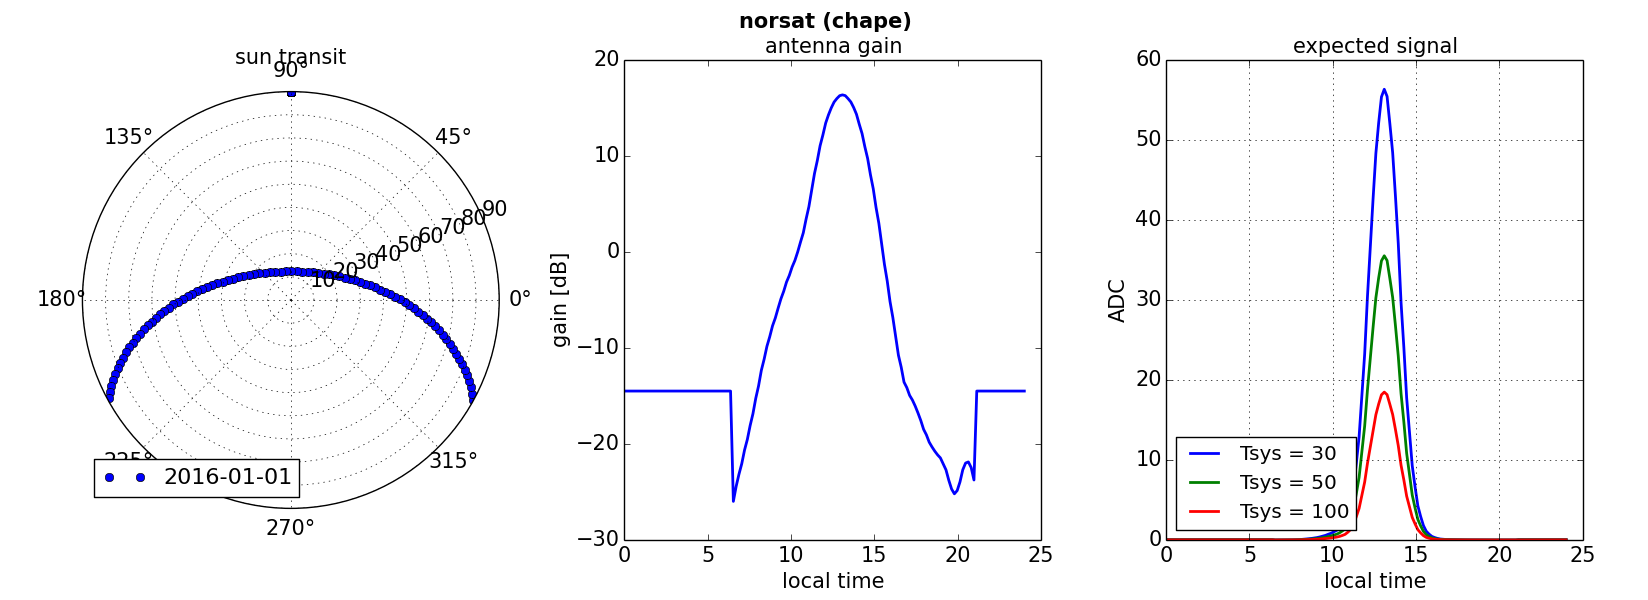
\includegraphics[width=0.7\linewidth]{expchape20160101.png}}\\
  \subfigure{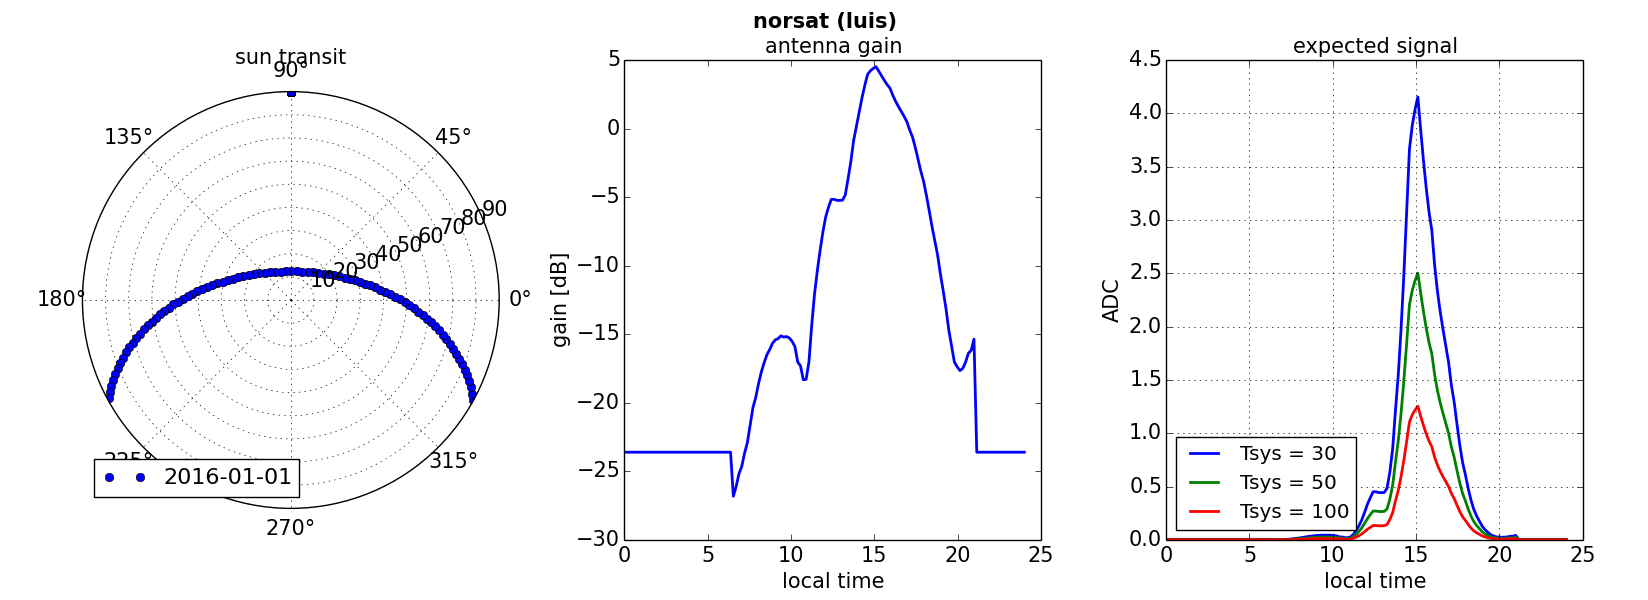
\includegraphics[width=0.7\linewidth]{expluis20160101.png}}\\
  \caption{Left: quiet sun spectrum, Right: varying component spectrum}
  \label{fig:spectra}
\end{figure}

\begin{figure}[!ht]
  \centering
  \hspace*{-3ex}
  \subfigure{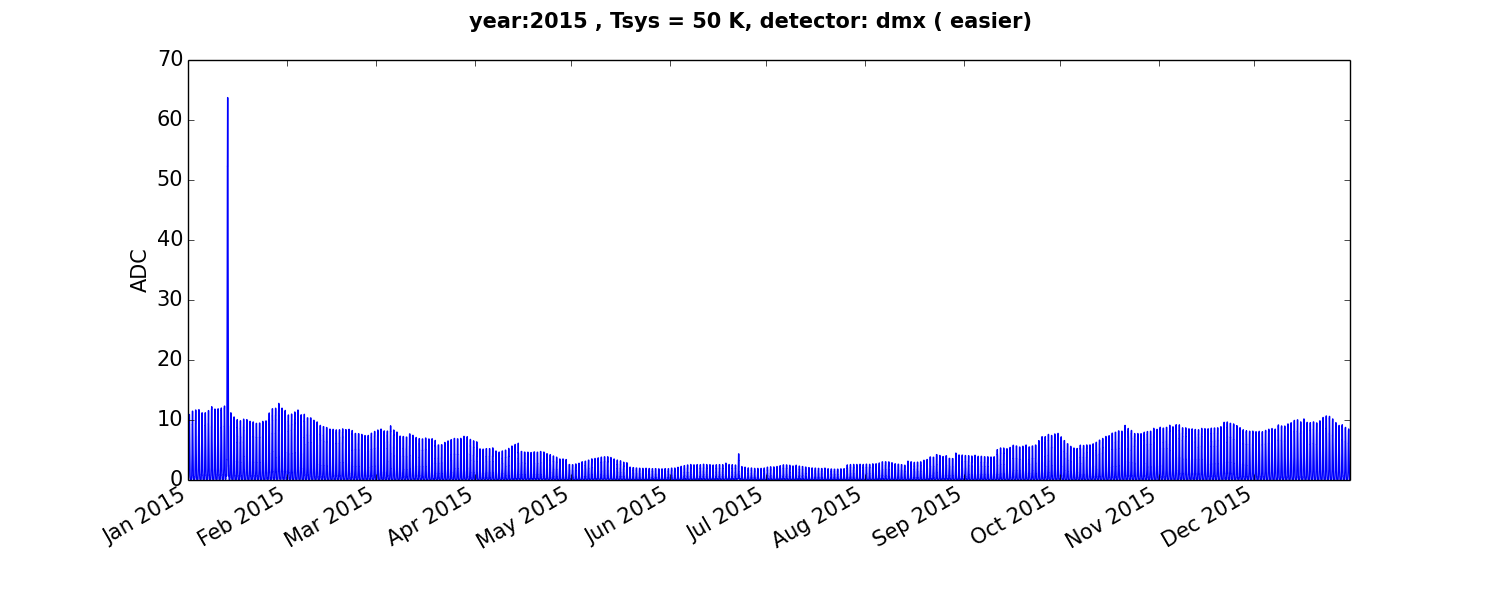
\includegraphics[width=0.7\linewidth]{year2015easier.png}}\\
  \subfigure{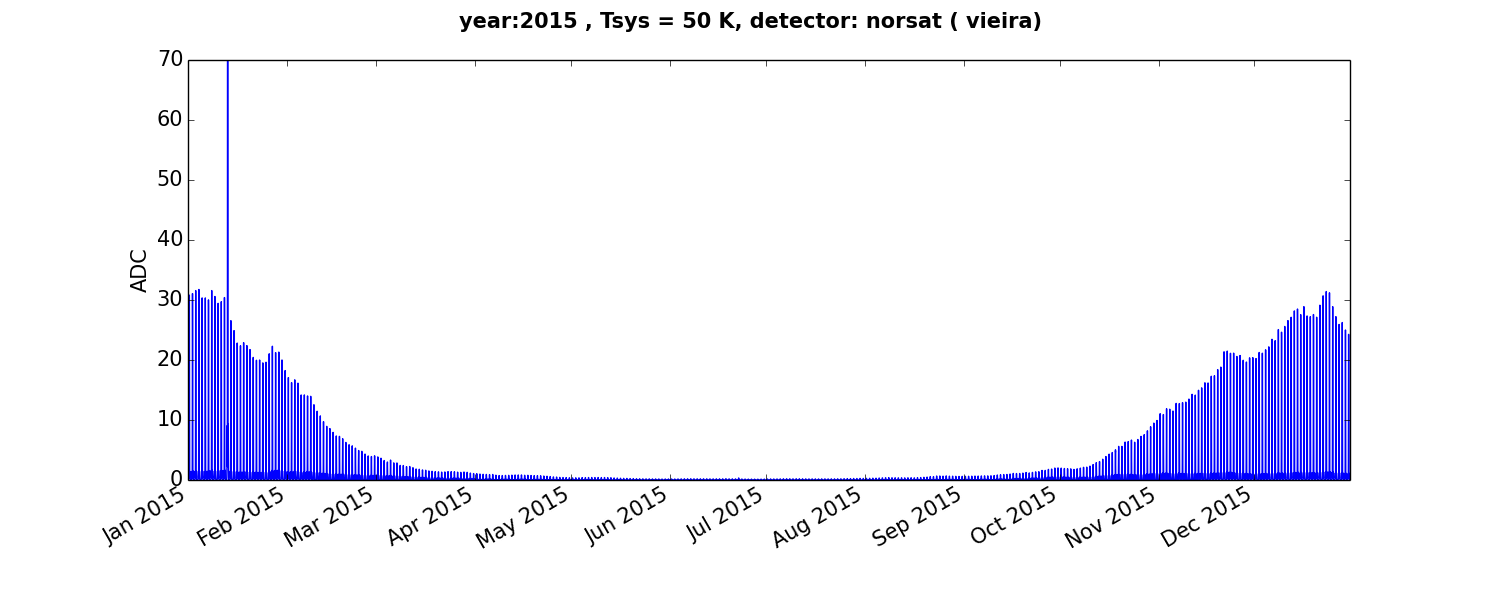
\includegraphics[width=0.7\linewidth]{year2015vieira.png}}\\
  \subfigure{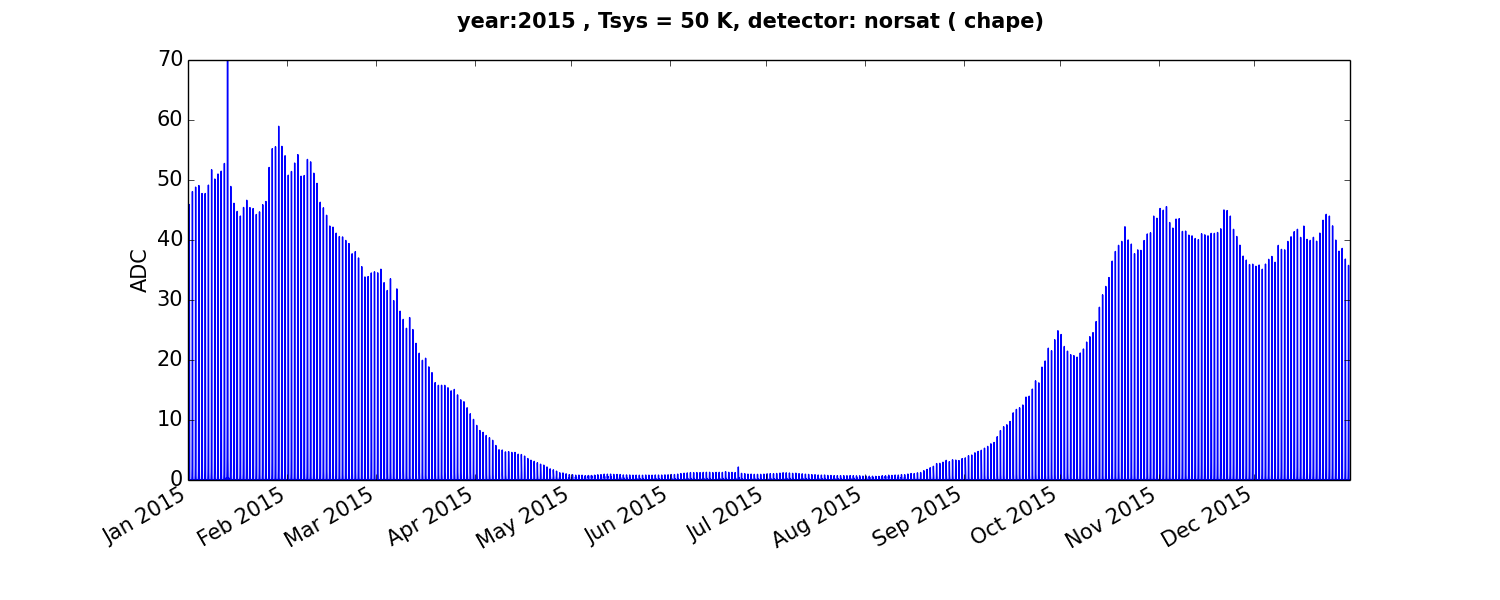
\includegraphics[width=0.7\linewidth]{year2015chape.png}}\\
  \subfigure{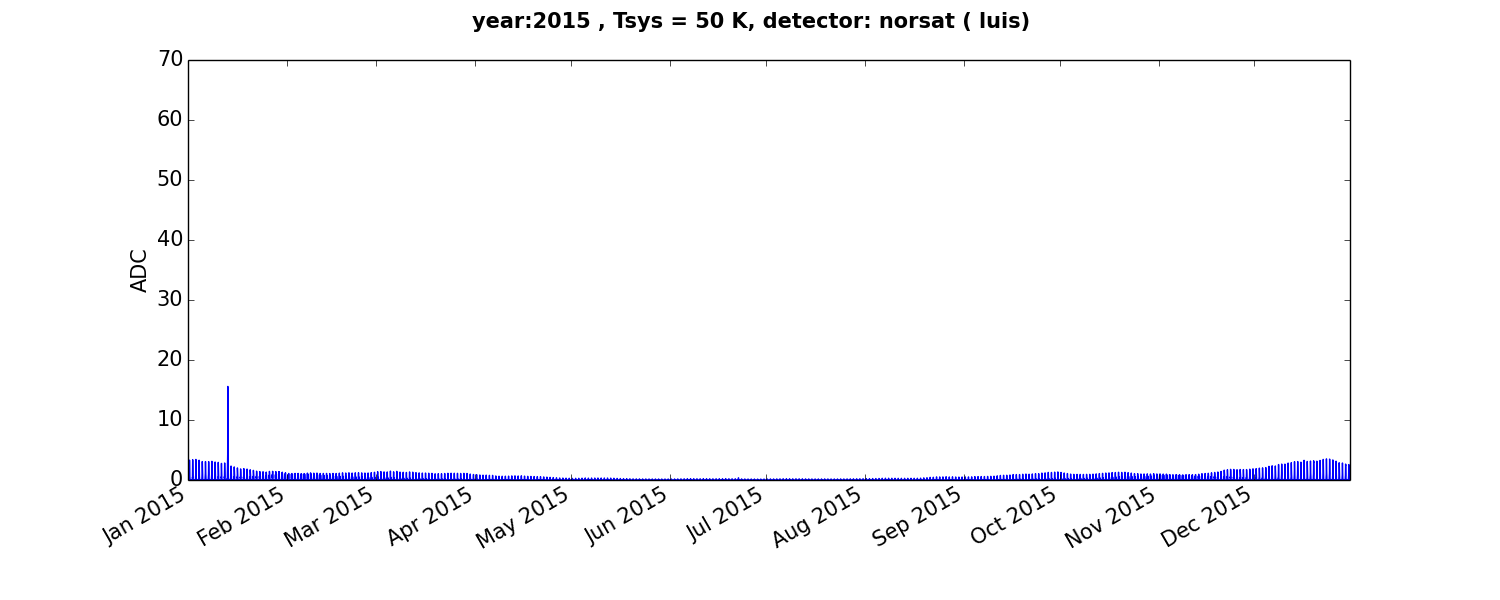
\includegraphics[width=0.7\linewidth]{year2015luis.png}}\\
  \caption{Left: quiet sun spectrum, Right: varying component spectrum}
  \label{fig:spectra}
\end{figure}



\section{GIGADuck}
\subsection{Data selection}
The  radio baseline  we  observe is  a  results of  several known  and
unknown effects. A daily modulation is due to the temperature and will
be corrected for in  section~\ref{sec:tempdep}.  Humidity can affect a
lot the baseline, but the  parameterization is more difficult. We also
notice some large change of the  baseline that are likely to be due to
storm.  We  present in this  section the cut  we operate to  clean the
data and keep  the period when the baseline is  mainly affected by the
temperature.\\In principle  we could make cuts on  humidity value, but
the  monitoring information  is not  always present.   We  operate the
selection only  the shape  of the radio  baseline and select  the days
when  the variations  are smooth.   The figure~\ref{fig:selectedpopey}
shows  the day  selected for  the  station Popey.   For instance,  the
period around  the 25th of March  was certainly a period  of rain, and
the  baseline of  Chape and  Popey is  affected, thus  this  period is
removed  from  the  dataset.   (The  date are  also  reported  in  the
appendix)
%% \begin{figure}[!ht]
%%   \centering
%%   \hspace*{-3ex}
%%   \subfigure{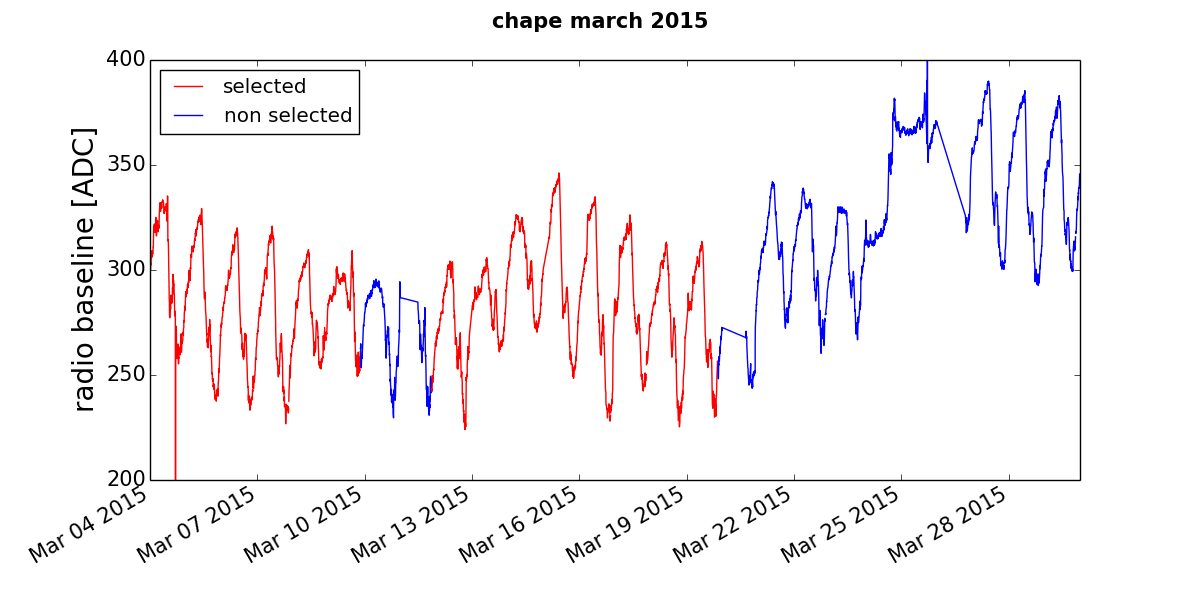
\includegraphics[width=0.49\linewidth]{chapemarch2015.png}}
%%   \subfigure{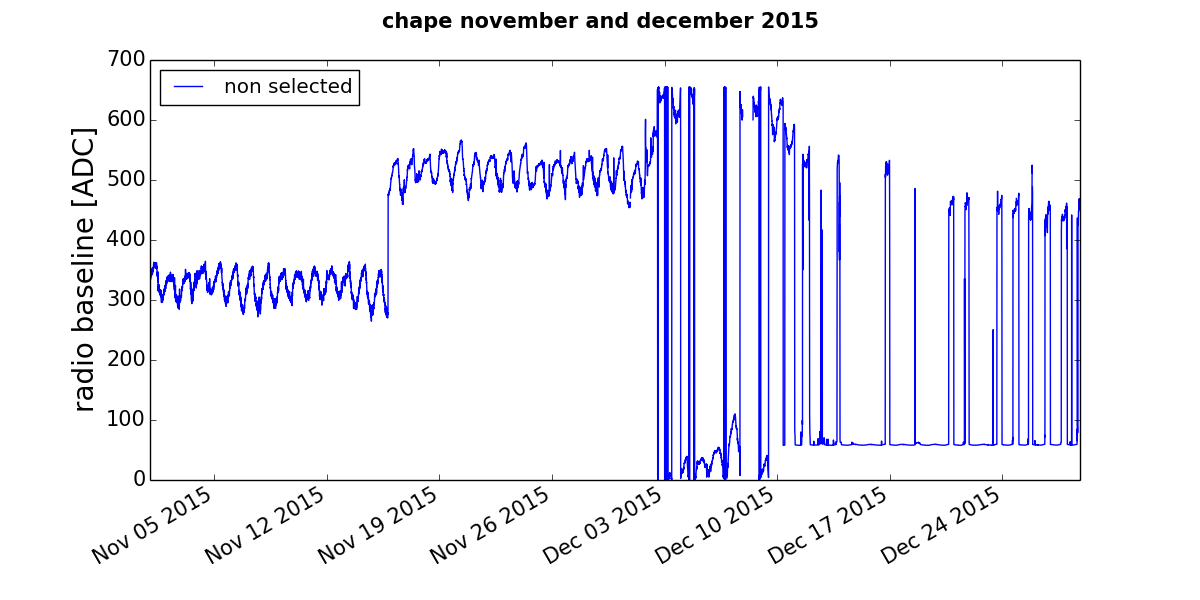
\includegraphics[width=0.49\linewidth]{chapenovdec2015.png}}\\
%%   \subfigure{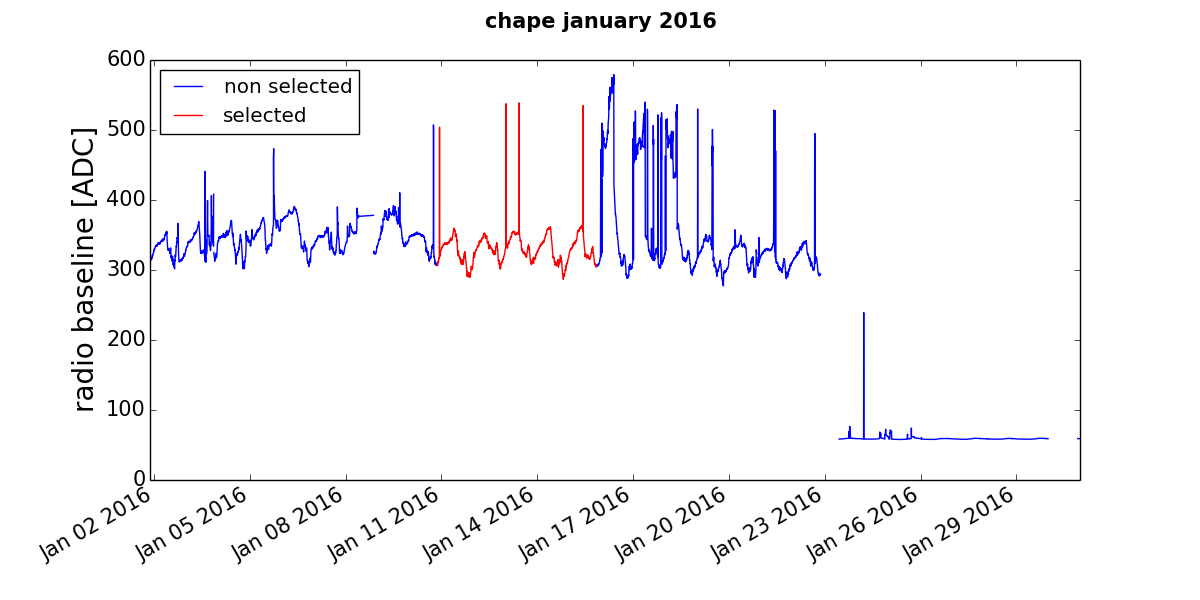
\includegraphics[width=0.49\linewidth]{chapejan2016.png}}
%%   \subfigure{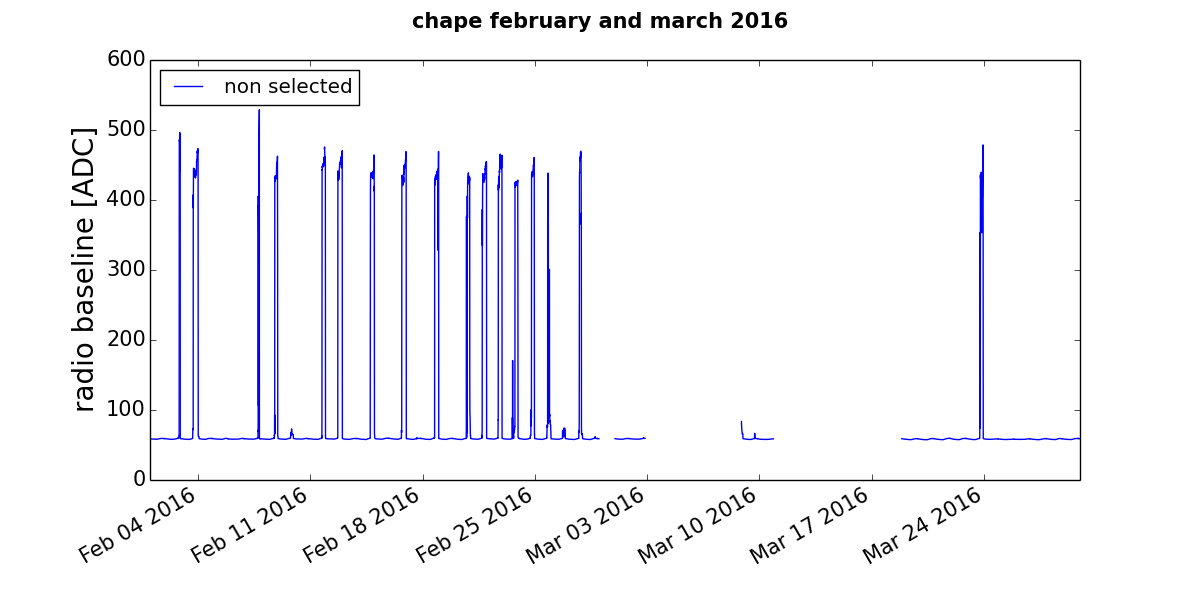
\includegraphics[width=0.49\linewidth]{chapefebmarch2016.png}}
%%   \caption{Radio baseline for four different periods for Chape station
%%     (id=384). In  red are the periods  kept for the  sun transit analysis
%%     based on the shape.}
%%   \label{fig:selectedchape}
%% \end{figure}

\begin{figure}[!ht]
  \centering
  \hspace*{-3ex}
  \subfigure{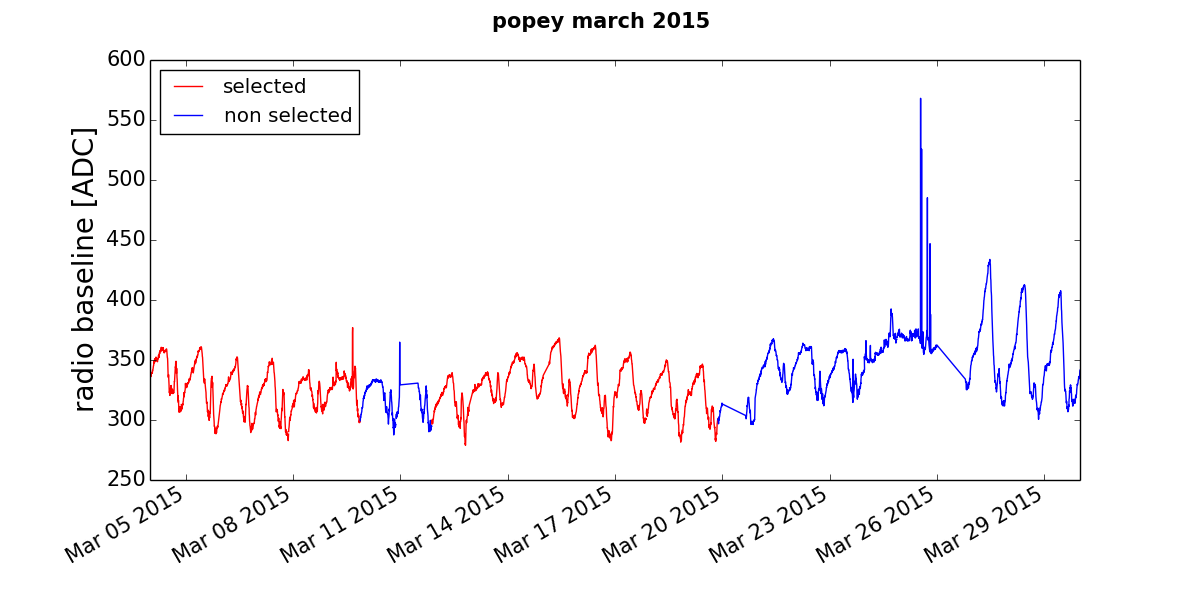
\includegraphics[width=0.49\linewidth]{popeymarch2015.png}}
  \subfigure{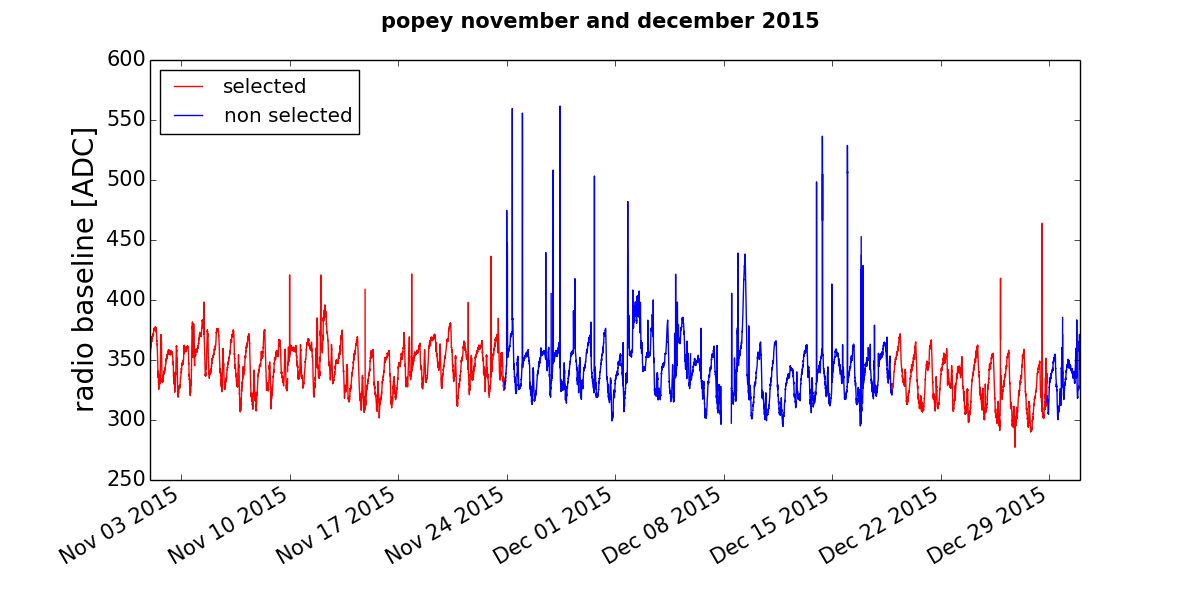
\includegraphics[width=0.49\linewidth]{popeynovdec2015.png}}\\
  \subfigure{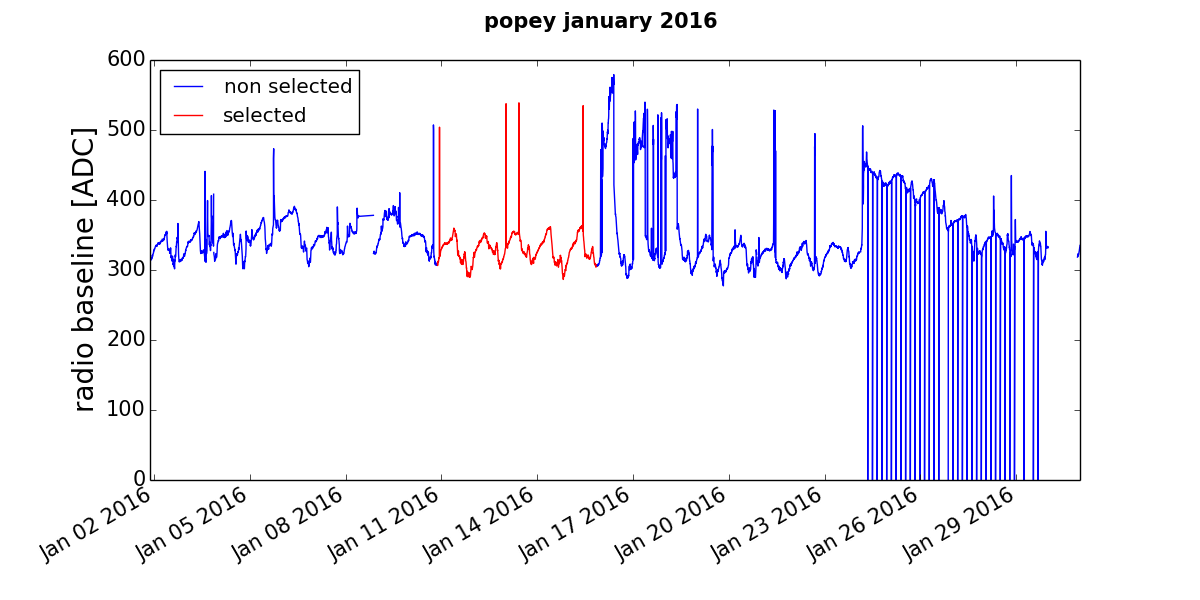
\includegraphics[width=0.49\linewidth]{popeyjan2016.png}}
  \subfigure{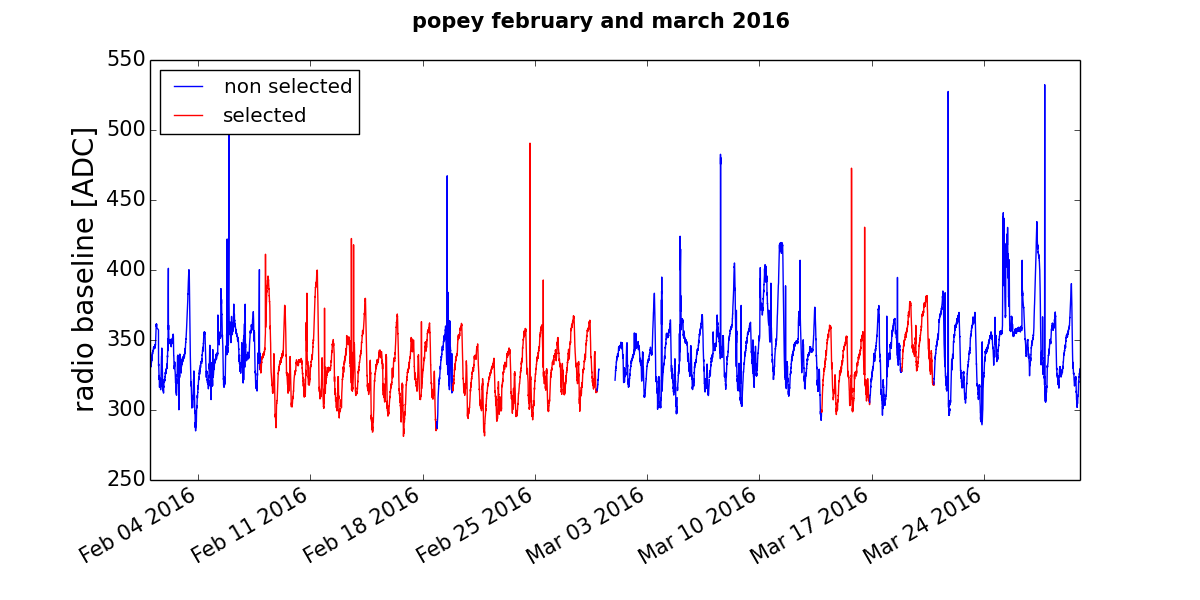
\includegraphics[width=0.49\linewidth]{popeyfebmarch2016.png}} 
  \caption{Radio baseline for four different periods for Popey station
    (id=385). In  red are the periods  kept for the  sun transit analysis
    based on the shape.}
 \label{fig:selectedpopey}
\end{figure}

\newpage
\subsection{Temperature dependence}
\label{sec:tempdep}  
The next step  is to correct from the effect  of temperature. First of
all we remove the time of the  day when the sun is expected (this time
depends on  the station because they point  toward different azimuth).
The  raw  plot  of  the  baseline  vs  temperature  is  shown  on  the
figure~\ref{fig:blvstempraw}.   For  Chape  we  notice  two  separated
populations. This is due to the  fact that we have sometimes a jump of
the baseline. To circumvent this  effect, we reference our data to the
daily average (see Figure~\ref{fig:blvstempmeansub}).  We parameterize
only the  variation of  the radio baseline  with the variation  of the
temperature:
\begin{itemize}
\item Chape: $\rm ADC - <ADC> = -2.93 (T - <T>) $
\item Popey: $\rm ADC - <ADC> = -3.67 (T - <T>) $ 
%\item Chape:  $\rm ADC - <ADC> = -2.93 (T - <T>)  -2.38\cdot10^{-5}$
%\item Popey: $\rm ADC - <ADC> = -3.67 (T - <T>)  -3.58\cdot10^{-6}$ 
\end{itemize}


\begin{figure}[!ht]
  \centering
  \hspace*{-3ex}
  \subfigure{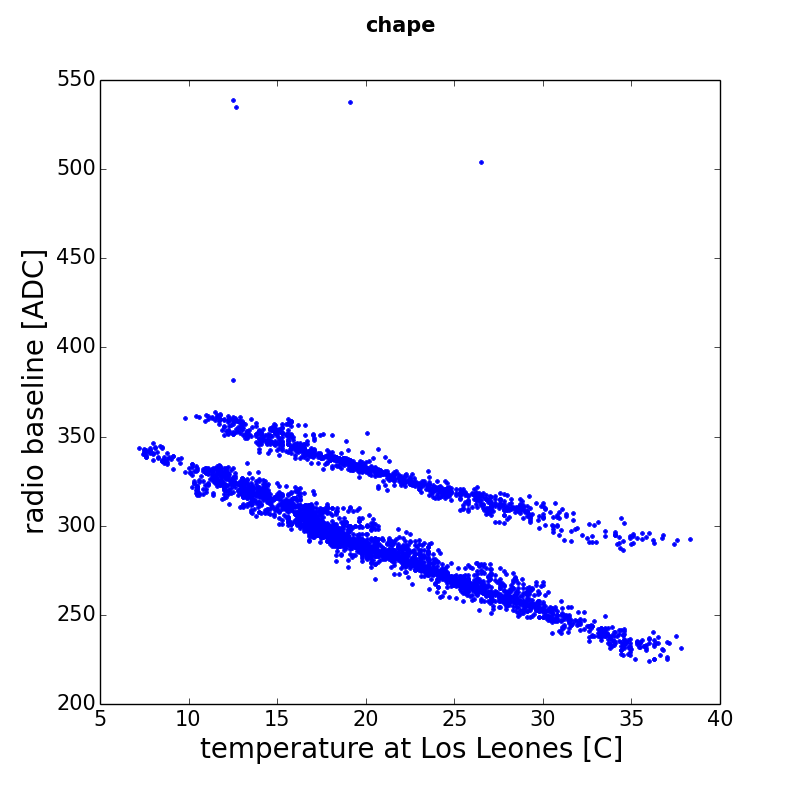
\includegraphics[width=0.49\linewidth]{chapeblvstempraw.png}}
  \subfigure{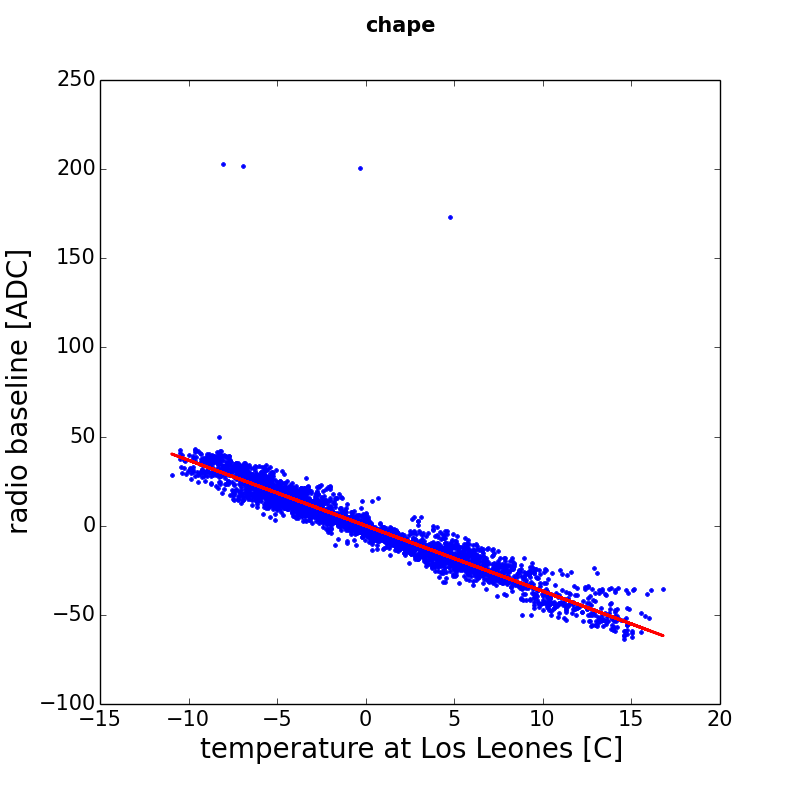
\includegraphics[width=0.49\linewidth]{chapeblvstempmeansub.png}}
  \caption{Selected period in red for Popey}
 \label{fig:blvstempraw}
\end{figure}

%% \begin{figure}[!ht]
%%   \centering
%%   \hspace*{-3ex}
%%   \subfigure{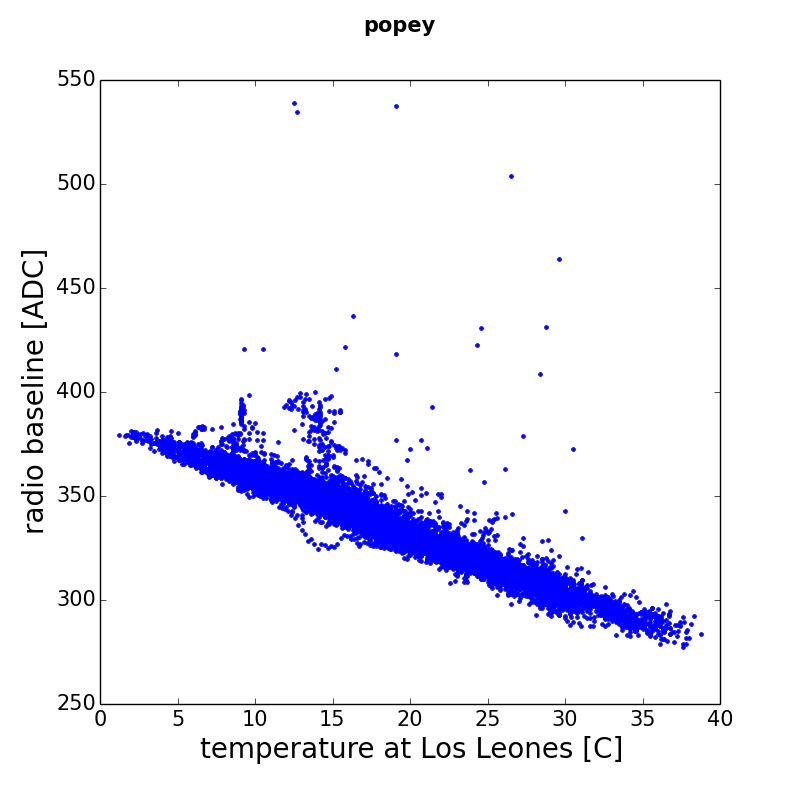
\includegraphics[width=0.49\linewidth]{popeyblvstempraw.png}}
%%   \subfigure{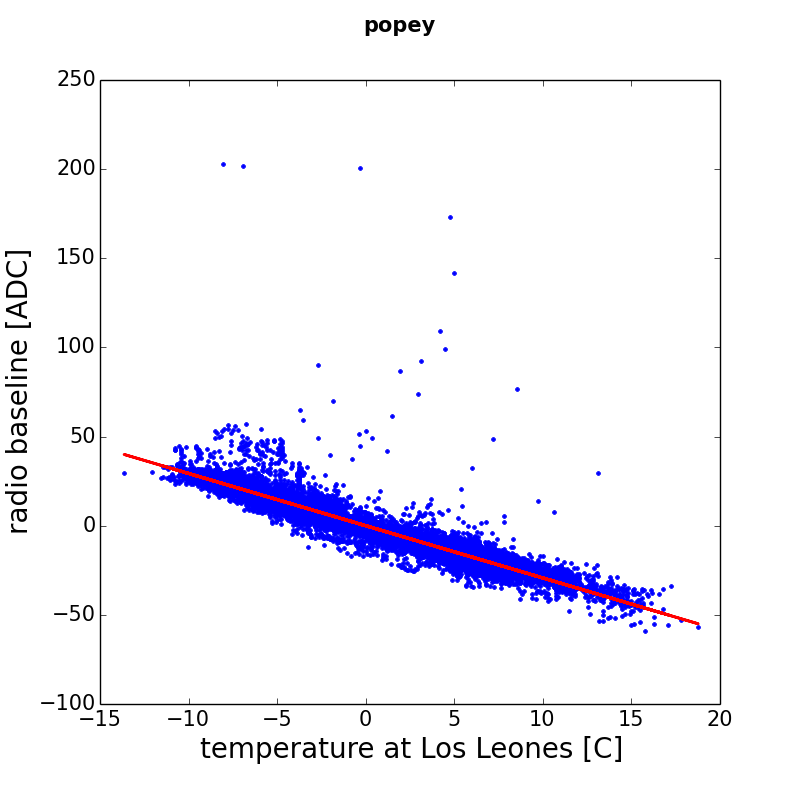
\includegraphics[width=0.49\linewidth]{popeyblvstempmeansub.png}}
%%   \caption{Selected period in red for Popey}
%%  \label{fig:blvstempmeansub}
%% \end{figure}

\subsection{Fit of the sun signal}
The temperature  correction removes the dominant  modulation.  The sun
signal is then fitted with a  Gaussian function. Example of such a fit
is shown in the  Figure~\ref{fig:examplefit}. A last selection is done
here on the fit output parameter. We remove the day when the fit value
of the time of maximum is more  than 1 hour away from the expected one
and the sigma of the gaussian is less than 20 minutes or more that 1.5
hour.
\begin{figure}[!ht]
  \centering
  \hspace*{-3ex}
  \subfigure{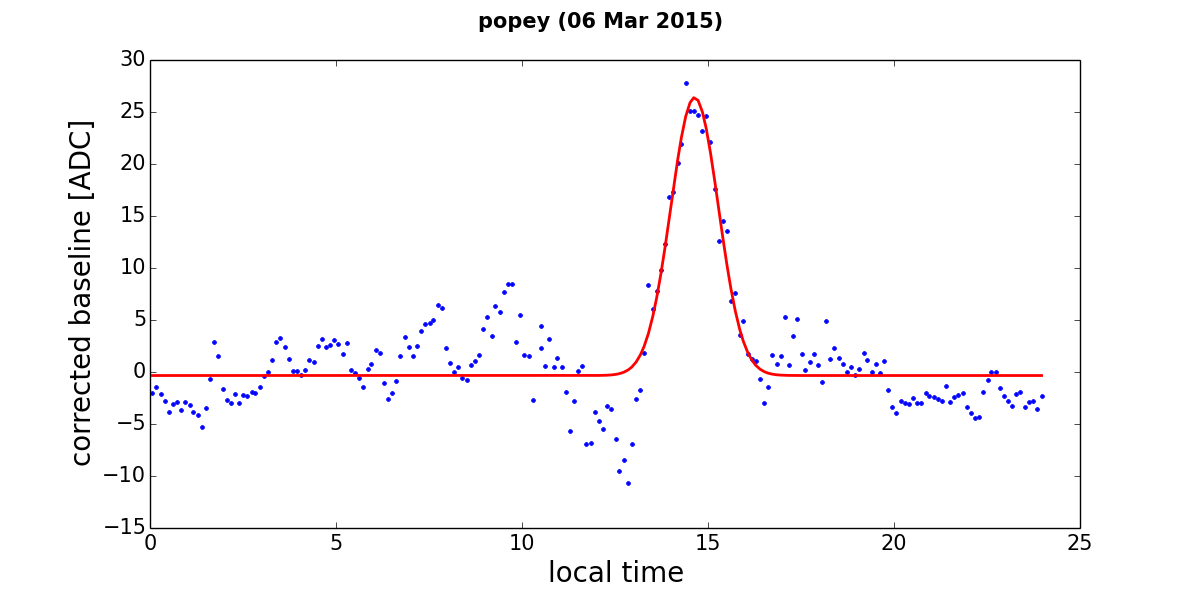
\includegraphics[width=0.49\linewidth]{fitexample.png}}
  \subfigure{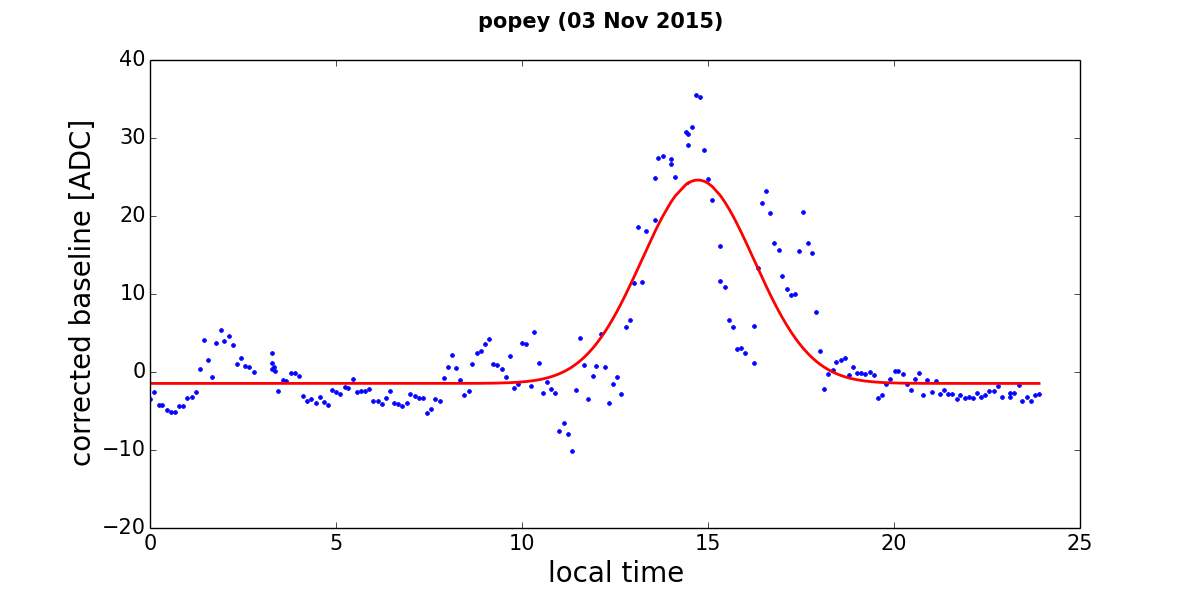
\includegraphics[width=0.49\linewidth]{badfitexample3.png}}
  \caption{Left: good fit example. Right: bad fit}
 \label{fig:examplefit}
\end{figure}
The formula used to retrieve the system temperature is:
\begin{equation}
  \rm
  T_{sys} (F_{sun}, A_{eff}, \Delta P) = \frac{\frac{1}{2} F_{sun} A_{eff}}{10^{\frac{\Delta P}{10}} -1 }
\label{eq:tsys}
\end{equation}
Where $\rm  F_{sun}$ is  the sun flux  measured by  other observatory,
$\rm A_{eff}$ is the effective area in the sun's direction, $\Delta P$
is the power difference in dB (with 1dB = 50 ADC count) and the factor
$\rm \frac{1}{2}$ is  the polarization factor. 

\subsection{Temperature measurement uncertainties}
From the  equation~\ref{eq:tsys}, we can compute  the uncertainties on
$\rm T_{sys}$:
\begin{equation}
  \rm       \sigma_{T_{sys}}^2      =      \frac{T_{sys}^2}{F_{sun}^2}
  \sigma_{F_{sun}}^2  + \frac{T_{sys}^2}{A_{eff}^2} \sigma_{A_{eff}}^2
  +   T_{sys}^2   \bigg(\frac{   \frac{\ln(10)}{10}   10^{\frac{\Delta
        P}{10}}}{10^{\frac{\Delta P}{10}}  - 1}\bigg)^2 \sigma_{\Delta
    P}^2
\end{equation}

\subsubsection{Sun flux uncertainties}
The  sun  flux  at  \unit[3.8]{GHz}  is  based  on  measured  data  at
\unit[2.8]{GHz}     and    the    parameterization     described    in
section~\ref{sec:expectedsignal}. We can  compare our results with the
Nobeyama  observatory data,  which collects  data on  the sun  flux at
\unit[2 and  4]{GHz} (we don't use  their data yet  because they don't
release  them   on  the  web).    The  figure~\ref{fig:sunflux}  shows
different fluxes:

\begin{figure}[!ht]
 \centering
 \hspace*{-3ex}
 \subfigure{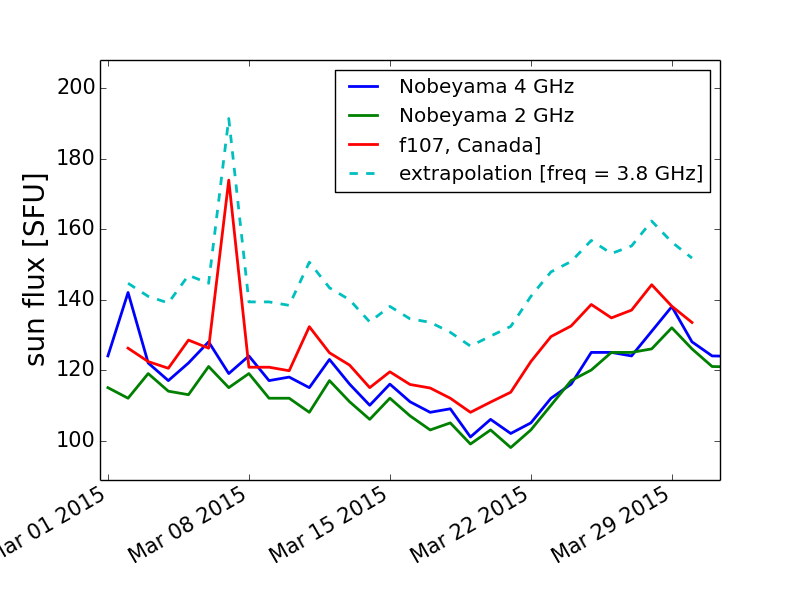
\includegraphics[width=0.49\linewidth]{sunfluxmarch.png}}
 \subfigure{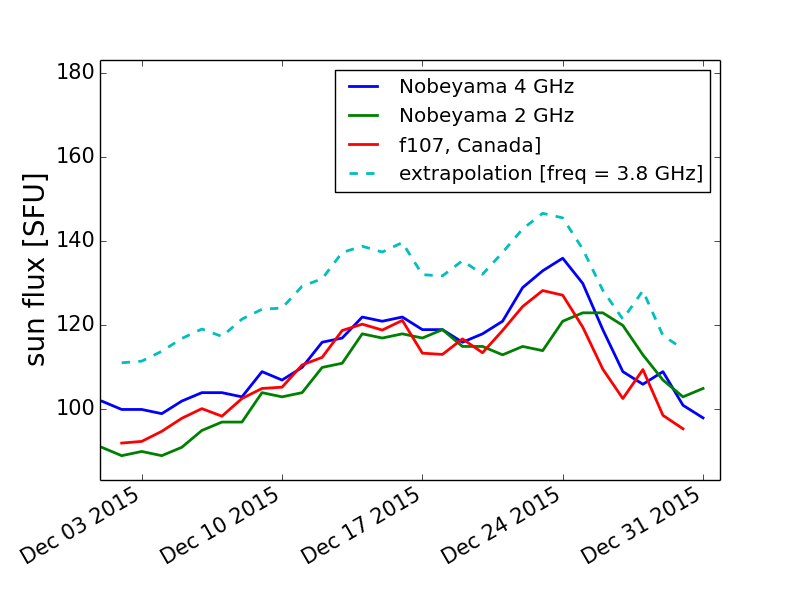
\includegraphics[width=0.49\linewidth]{sunfluxdec.png}}
%% \subfigure{\includegraphics[width=0.49\linewidth]{sunexpected.png}}
 \caption{sun flux for at different frequencies}
%%    Simulated  baseline  increase for  three  antennas  during the  sun
%%    passage.}
 \label{fig:sunflux}
\end{figure}
The value reported on the plots for the Nobeyama observatory are taken
from what is  displayed on their daily curves. I  don't really know if
this is an  average or the minimum value.  In any  case, the values at
\unit[2 and  4]{GHz} are lower than  what is measured  at the Canadian
site~\cite{sundata,  sundata2} by around  20\%. Since  I am  still not
sure of the meaning of the value for the Nobeyama data, I will account
for   an  uncertainty   of   20\%  in   the  temperature   calculation
(\textbf{this has to be improved either by taking the data of Nobeyama
  or by determining a precise uncertainty.}). 20\% corresponds also to
the precision given for the used parameterization~\cite{sunparam}.

\subsubsection{Effective area uncertainties}
Our measurement contains  an uncertainty on the effective  area, be it
because  of the  pointing direction  or our  limited knowledge  of the
gain.  We  only account  the possible shift  in zenith angle,  since a
shift in azimuth  would mainly affect the time  of maximum and slighly
the  amplitude of  the  signal.   We estimate  the  possible shift  in
pointing to  2$\rm ^{\circ}$.  The  resulting uncertainty on  the gain
depends   on   the   zenith   angle   at   the   sun   maximum.    The
Figure~\ref{fig:aeffuncert}  (left) shows  the antenna  effective area
and a  Gaussian fit as a  function of the zenith  angle. The resulting
uncertainties  on  the  effective   area  is  based  of  the  Gaussian
parameters   and    its   angle    dependence   is   shown    on   the
Figure~\ref{fig:aeffuncert} (right).

\begin{figure}[!ht]
 \centering
 \hspace*{-3ex}
 \subfigure{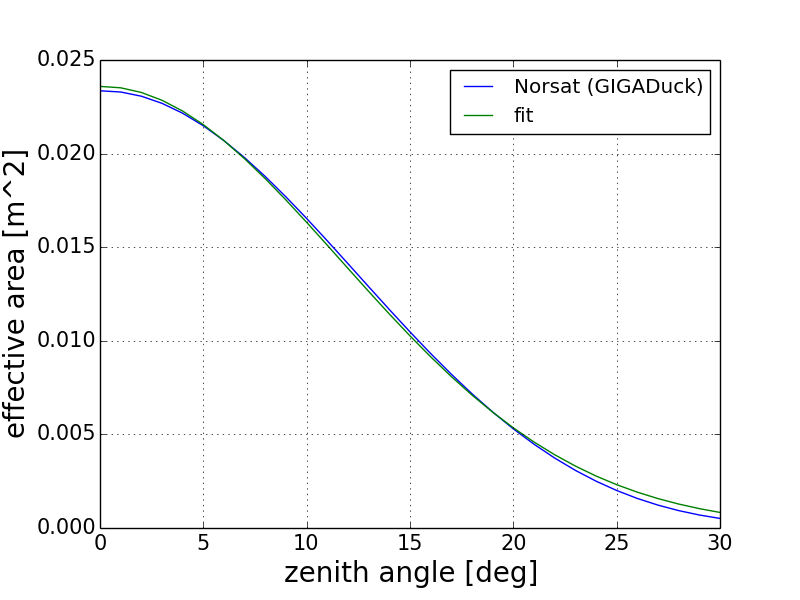
\includegraphics[width=0.49\linewidth]{aeff.png}}
 \subfigure{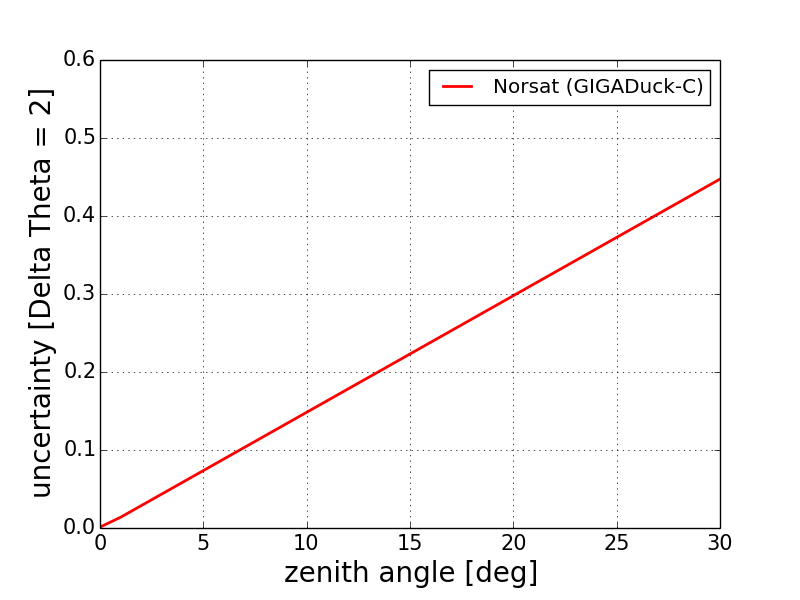
\includegraphics[width=0.49\linewidth]{sigmaaeff.png}}
 \caption{Effective  area of  the AInfo  antenna from  HFSS simulation
   (blue), Gaussian  fit (green).  Right: relative uncertainty  on the
   effective area}
 \label{fig:aeffuncert}
\end{figure}
We perform the  temperature measurement only during the  months when a
significant signal  from the  sun is expected,  that means when  it is
high in the  sky. The zenith angle at which the  sun signal is maximum
(in the  simulation) is shown in  the figure~\ref{fig:zenithofmax} for
three  antenna: Vieira  the central  detector  that points  up to  the
zenith,  Chape and  Orteguina (see  figure~\ref{fig:sunsim}  for their
field of view).
\begin{figure}[!ht]
 \centering
 \hspace*{-3ex}
 \subfigure{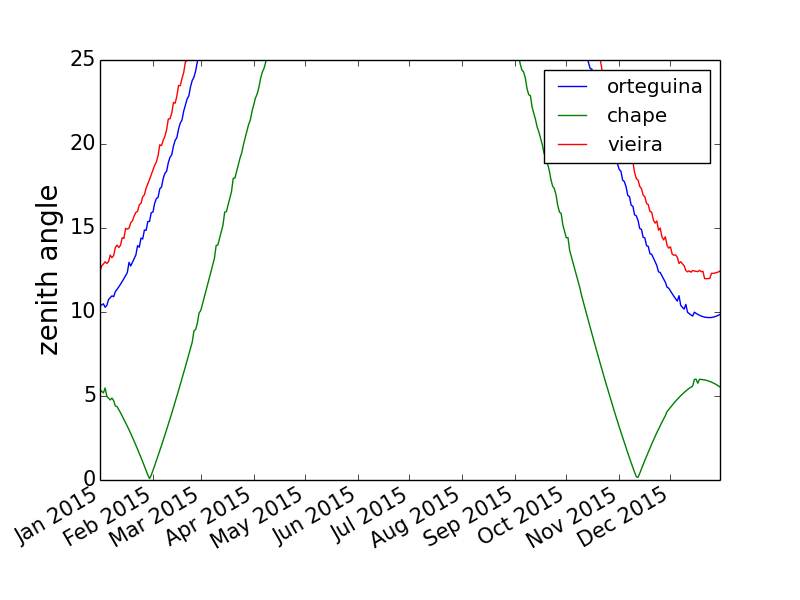
\includegraphics[width=0.49\linewidth]{zenithofmax.png}}
 \caption{Zenith angle when the sun signal is maximum as a function of
   the date}
 \label{fig:zenithofmax}
\end{figure}
The angle at  which the sun is observed when the  signal is maximum is
below  \unit[10]{$\rm  ^{\circ}$} for  Chape  but  around \unit[15  to
  20]{$\rm  ^{\circ}$}   in  March  for  Vieira   or  Orteguina.  This
translates to an uncertainty that can reach up to 40\%.


\subsubsection{Uncertainty on $\rm \Delta P$}
The uncertainty  on the  measured power induced  by the sun  flux $\rm
\Delta P$ comes from our ability to measure a variation of baseline on
an hour time scale.  The process to estimate this variation, summed up
in section~\ref{sec:tempmeas}, is based on  a fit of the sun bump with
a  Gaussian   function  and  the   background  with  a   second  order
polynominals.   There  aren't   actually  any  justification  for  the
background fit. To estimate the error on the $\rm \Delta ADC$ we make,
we  change the fitting  method and  see how  the results  change.  The
figure~\ref{fig:fits}  shows the  results  of $\rm  \Delta  ADC$ as  a
function  of  the date  when  the baseline  is  either  fitted with  a
constant  and a  Gaussian  or with  a  second order  polynomial and  a
constant, on  the right side  is shown the corresponding  histogram of
the difference of the two methods.

%\section{Data description and baseline parameterization}
In this  section we attempt  to understand and parameterize  the radio
baseline.      We     will     separe    the     various     detectors
EASIER7/EASIER61/GIGADuck.  The first part  describes the basic cut we
apply,  the  second describes  the  baseline  parameterization we  can
obtain.  We analyse  the monitoring data recorded every  400 second at
the local  station.  The  data contains the  basic information  on the
radio  trace,  i.e.   the average  and  the  RMS.   But we  have  also
information  from the  Los Leones  weather station,  for  instance the
outside temperature and humidity.
\newpage
\subsection{a first look at the data and basic cuts}
We expect the radio baseline to vary because of different sources:
\begin{itemize}
\item a  variation of gain:  a variation of  gain is likely  to happen
  with temperature.
\item  the microwave flux:  if a  source strong  enough enters  in the
  field of view  of the antenna. This is what is  expected for the sun
  flux.
\item atmospheric effect:  this is also a variation  of the radio flux
  but it is  due to absorption of clouds, or an  increase of the field
  due to stormy conditions.
\end{itemize}
\subsubsection{overview}
We  show   the  raw   baseline  over  several   time  scales   in  the
figure~\ref{fig:scales}.
\begin{figure}[!ht]
  \centering
  \hspace*{-3ex}
  \subfigure{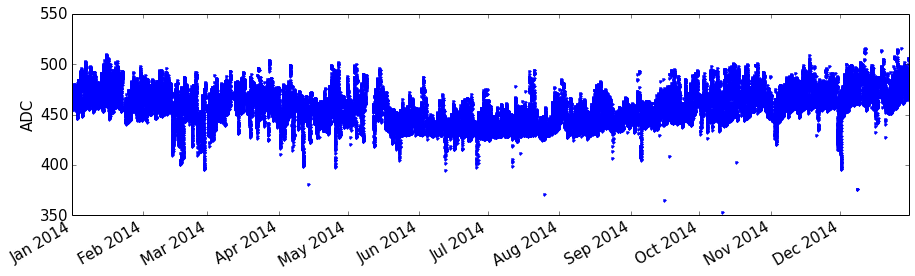
\includegraphics[width=0.9\linewidth]{oneyear.png}}\\
  \subfigure{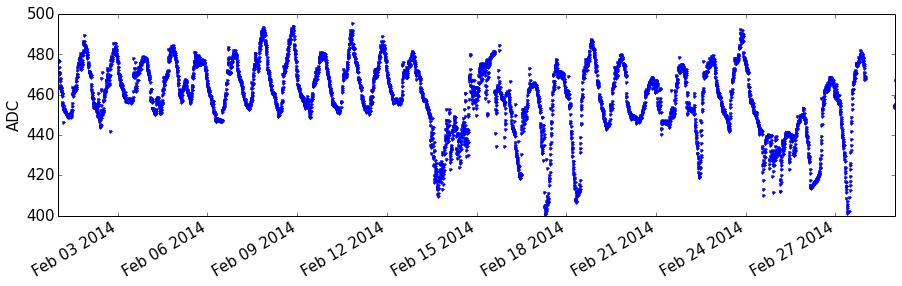
\includegraphics[width=0.9\linewidth]{onemonth.png}}\\
  \subfigure{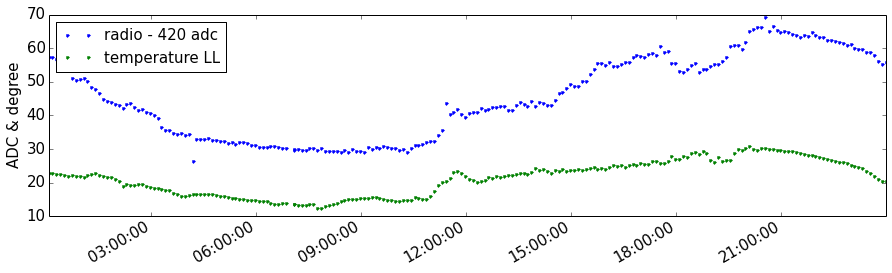
\includegraphics[width=0.9\linewidth]{oneday.png}}
  \caption{Left: quiet sun spectrum, Right: varying component spectrum}
  \label{fig:scales}
\end{figure}
We see  two main modulations,  a long term  variation one on  the year
long plot, and a daily modulation  on the month long plot. We can also
notice a  large decrease of the  baseline (i.e. increase  of the radio
power) for instance in the middle  of February. We will see later that
this can be related to rain. When there is no such rainy condition the
typical spread of the baseline  is around 40-50 ADC counts. However we
notice  clearly  on the  bottom  plot  of figure~\ref{fig:scales}  the
strong dependence with the outside temperature. \\ When we compare the
7     antennas     over      the     same     time     period     (see
figure~\ref{fig:allantennas}),  we notice the  structure has  the same
shape, but the amplitude of  the variations can be very different: for
instance stId332 has  variations of the order of  30-40 ADC counts and
stId 342 has variations of the order of 150 ADC counts)
\begin{figure}[!ht]
  \centering
  \hspace*{-3ex}
  \subfigure{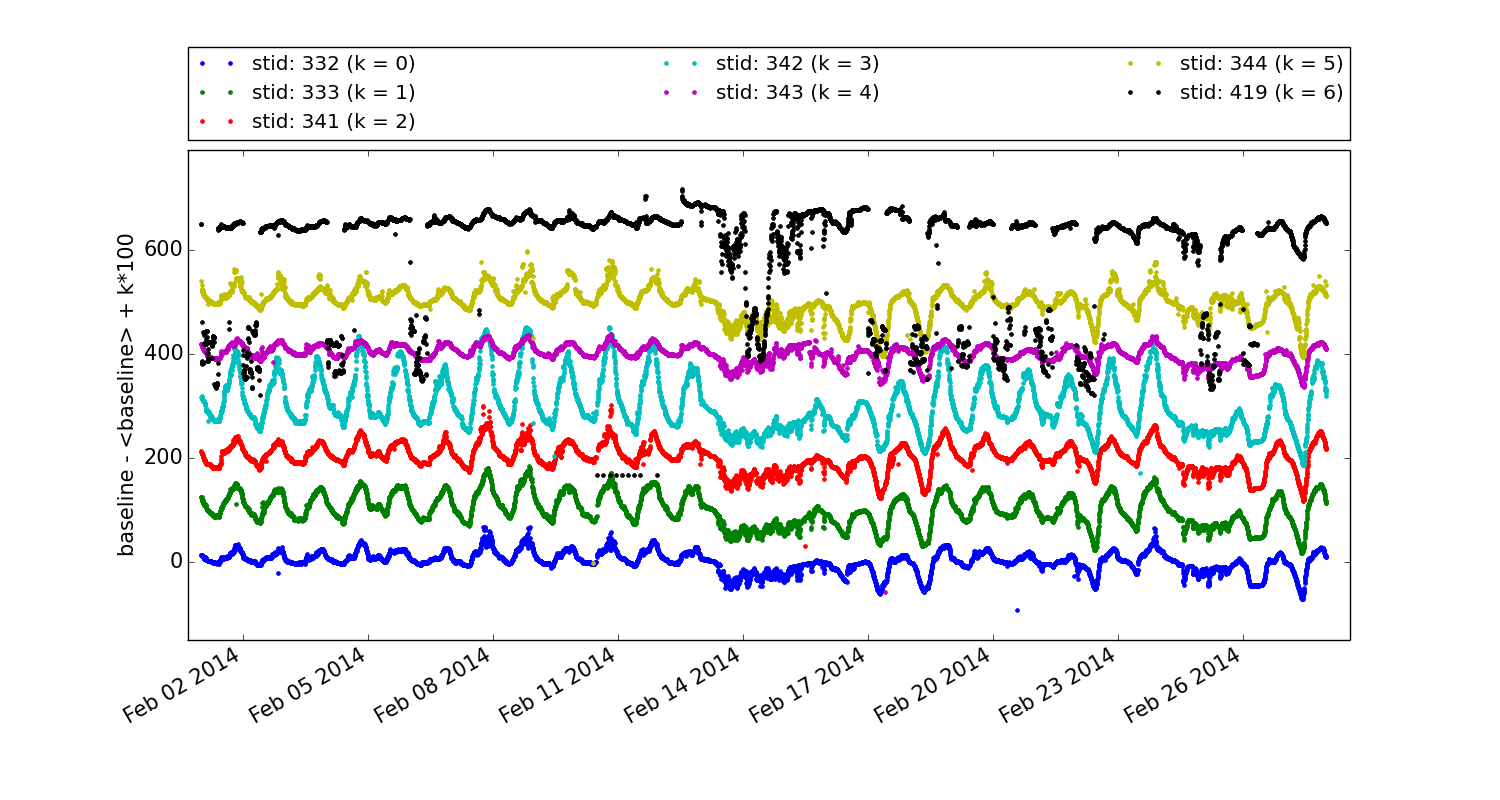
\includegraphics[width=0.9\linewidth]{allantennas.png}}
  \caption{}
  \label{fig:allantennas}
\end{figure}
In my opinion, these differences  are due to a different dependence of
the gain with the temperature.  The  gain itself is not related to the
system temperature, but it shows  that the 7 LNBf might have different
characteristics.
\subsubsection{cuts}
\paragraph{humidity}
We  have just  seen that  some periods  look very  different,  see for
instance around  February 15 in the  fig~\ref{fig:scales}. These large
baseline seem  to be related to the  rain.  Figure~\ref{fig:rain} show
the baseline  together with the humidity percentage  measured with Los
Leones weather station. It is  clear that a humidity larger than 60/70
\%  has a  strong  effect on  the  baseline.  This  effect  is more  a
threshold effect than a correlation:  when it rains we can't trust the
baseline.
\begin{figure}[!ht]
  \centering
  \hspace*{-3ex}
  \subfigure{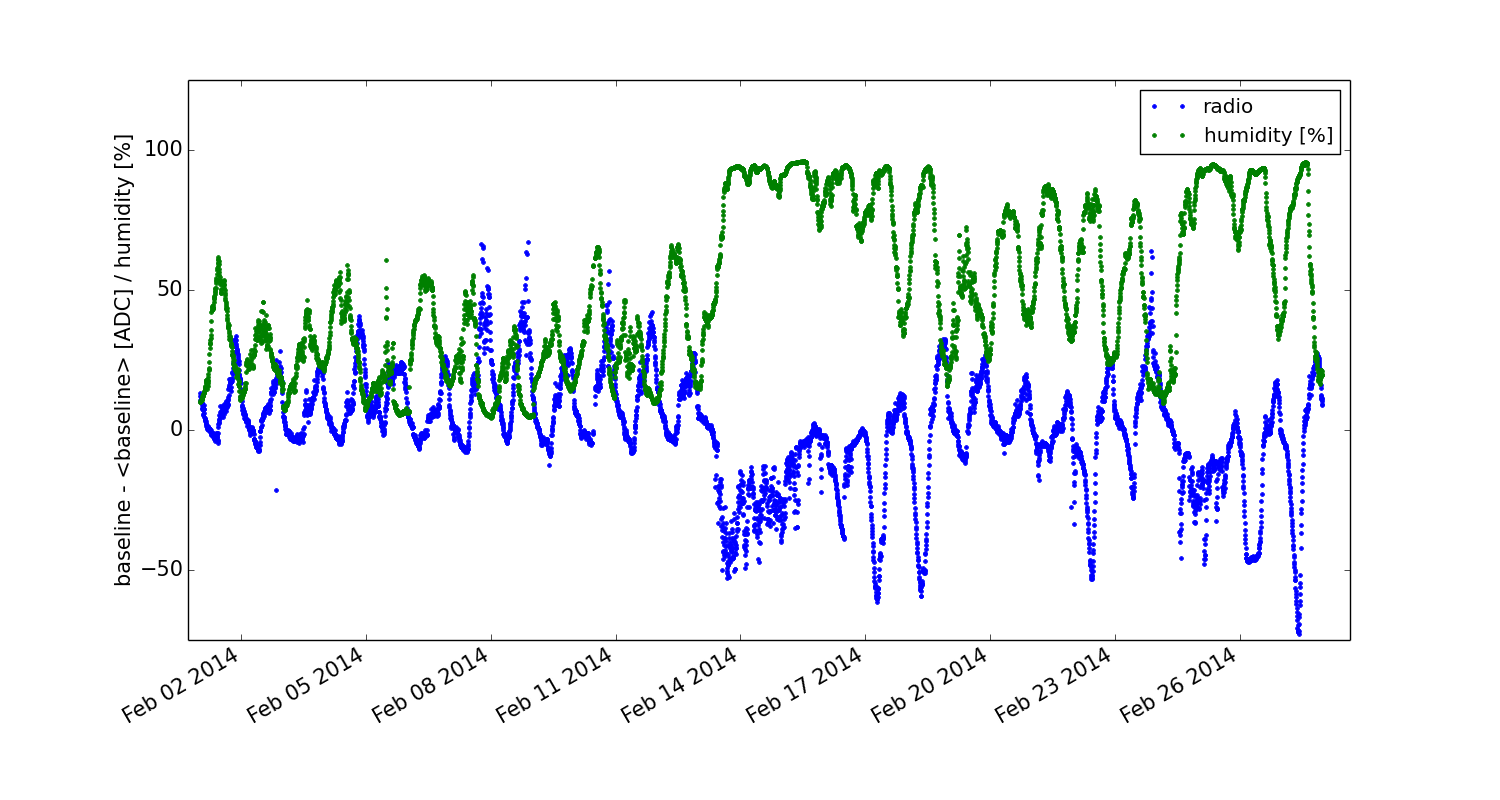
\includegraphics[width=0.9\linewidth]{radiohum.png}}
  \caption{}
  \label{fig:rain}
\end{figure}
In the following we require the humidity to be less than 50 \%.


\paragraph{sun/no sun periods}
The sun is expected to give a contribution to the baseline. We need to
exclude the period  when a significant signal is  expected in order to
keep  this effect.   The sun/no  sun periods  are determined  with the
expected signal calculated  above. We assume a temperature  of 50K for
the detector and  consider a signal above 5  ADC count as significant.
The figure~\ref{fig:sunnosun} is  an example of the split  of the data
in sun/no sun period (also after the humidity cut). 
\begin{figure}[!ht]
  \centering
  \hspace*{-3ex}
  \subfigure{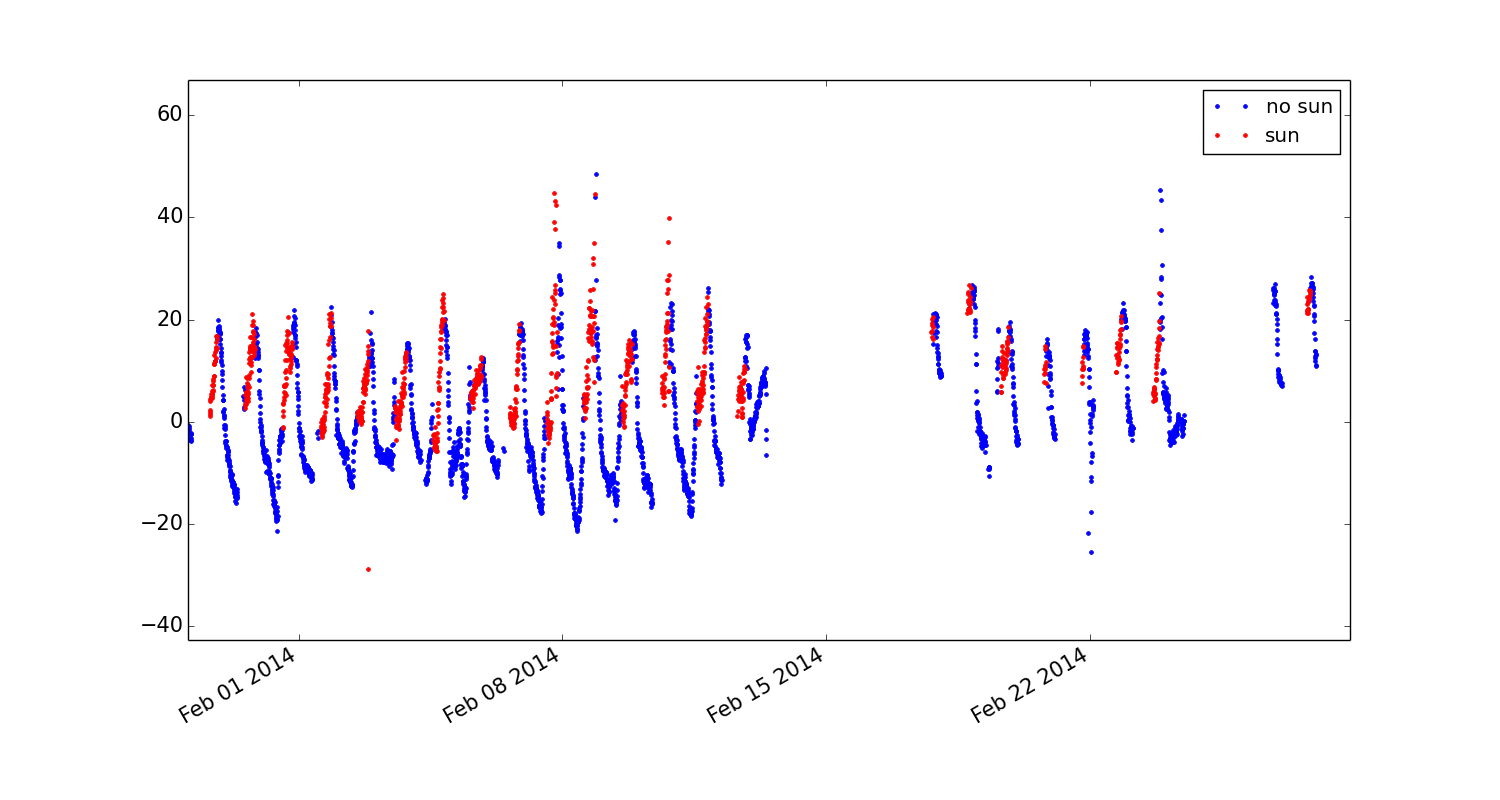
\includegraphics[width=0.49\linewidth]{sun_nosun.png}}
  \subfigure{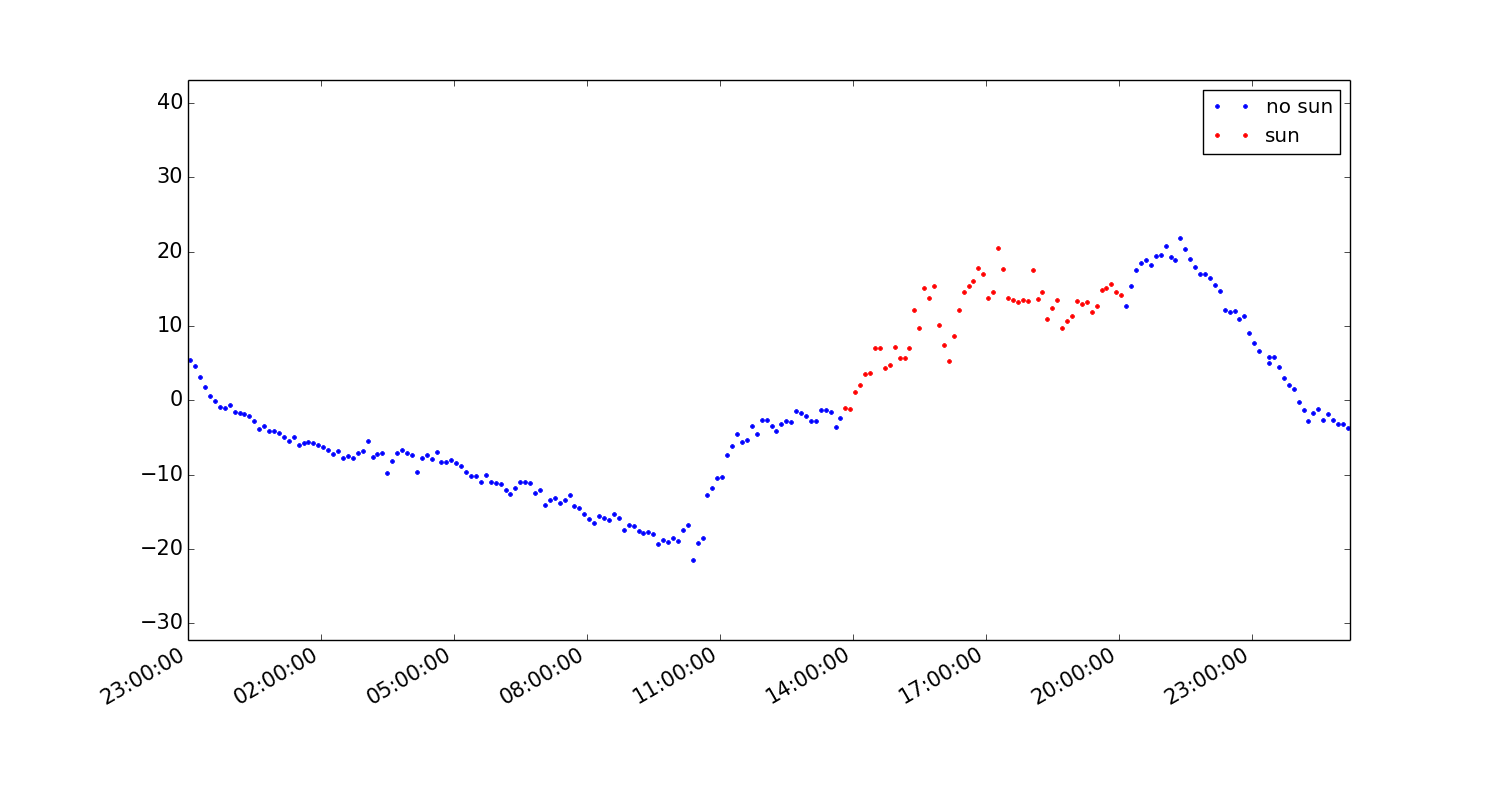
\includegraphics[width=0.49\linewidth]{sun_nosun2.png}}
  \caption{}
  \label{fig:sunnosun}
\end{figure}
\paragraph{long term variation}
We have seen that there is  a long term modulation of the baseline. To
remove this  dependence we filter  out the low frequencies  (below one
day). 

\subsection{Temperature parameterization}
The   radio   baseline   is   strongly  dependent   on   the   outside
temperature. The figures~\ref{fig:ybltemp}  shows the baseline against
the temperature for one year of data of the stations 332 and 342. This
can be explained  by a variation of the LNB  gain with the temperature
\cite{PStempnote}.   When we  perform  a linear  fit  and correct  the
baseline with this function, we  obtain a baseline distribution with a
spread of 5 to 16 ADC depending on the station.
\begin{figure}[!ht]
  \centering
  \hspace*{-3ex}
  \subfigure{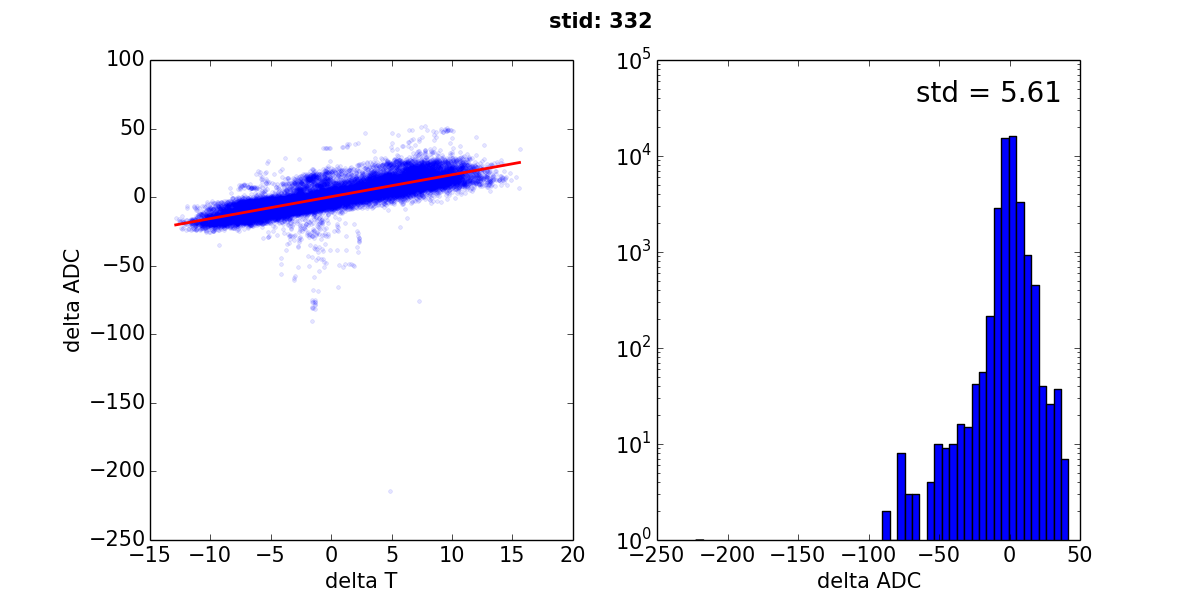
\includegraphics[width=0.9\linewidth]{yfit332.png}}\\
  \subfigure{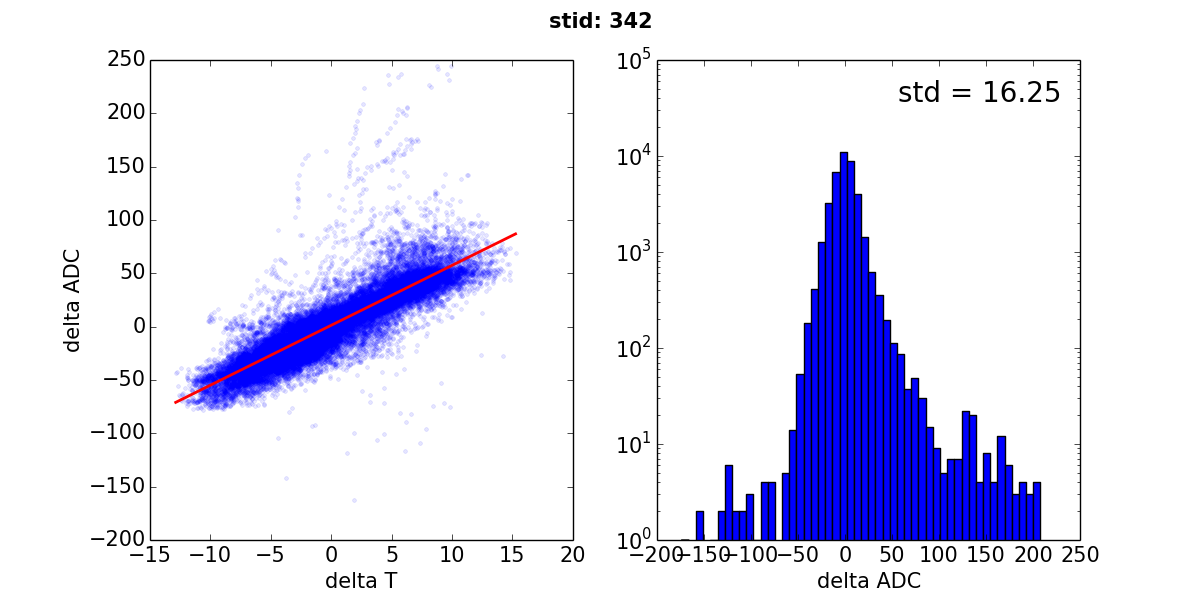
\includegraphics[width=0.9\linewidth]{yfit342.png}}
  \caption{}
  \label{fig:ybltemp}
\end{figure}

If we perform a daily fit  of the temperature dependence we can obtain
a   better   correction   of   the   baseline.    We   show   in   the
figure~\ref{fig:dbltemp} the  fits for  each day on  the left  and the
resulting corrected distribution on the right. 
\begin{figure}[!ht]
  \centering
  \hspace*{-3ex}
  \subfigure{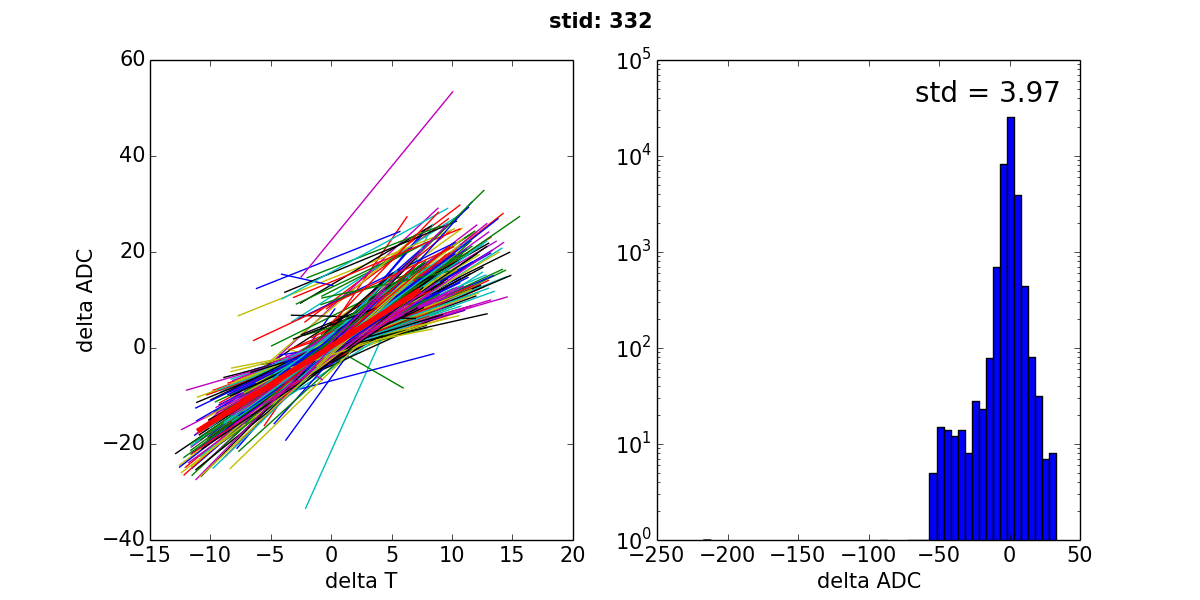
\includegraphics[width=0.9\linewidth]{dfit332.png}}\\
  \subfigure{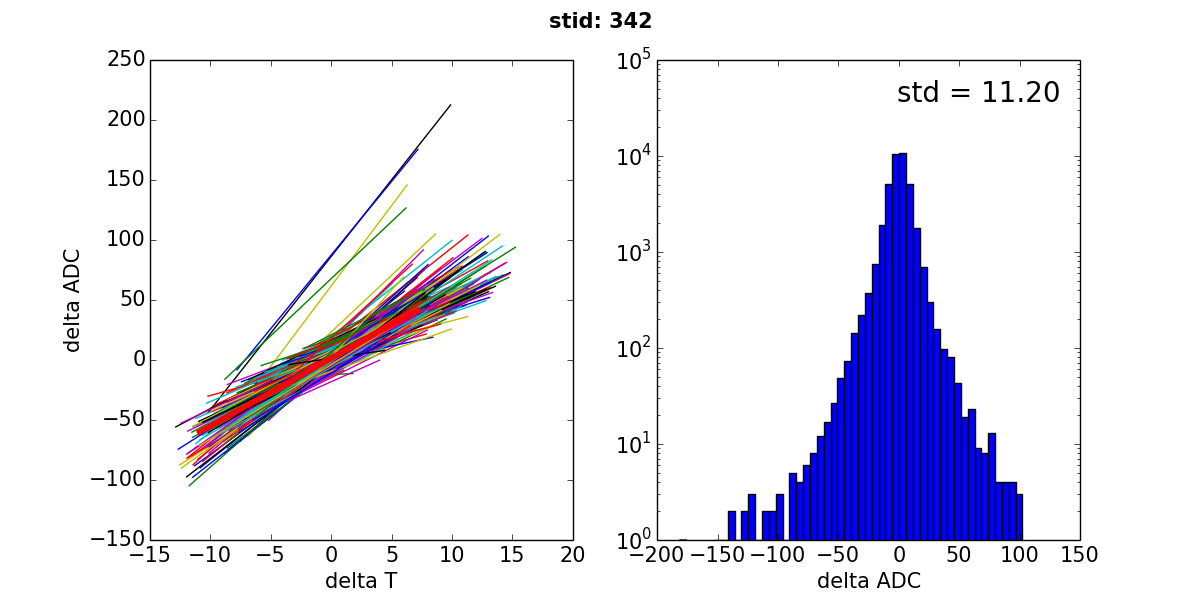
\includegraphics[width=0.9\linewidth]{dfit342.png}}
  \caption{}
  \label{fig:dbltemp}
\end{figure}
We  see that  the fits  can be  very different  depending on  the day,
meaning that other parameters are not accounted for. \\Furthermore, we
want  to be  able  to compare  a  \textit{non sun}  hypothesis with  a
\textit{sun}  hypothesis, so  we  need a  prediction  of the  baseline
during the time we expect the sun ( the sun signal is expected usually
between  11h00 and  16h00  in local  time,  i.e.  14h00  and 19h00  in
UTC).  In  the   figure~\ref{fig:prediction1}  we  show  the  baseline
comparison of  the baseline  between 14:00 and  19:00 for the  days we
don't expect the sun  signal. 
\begin{figure}[!ht]
  \centering
  \hspace*{-3ex}
  \subfigure{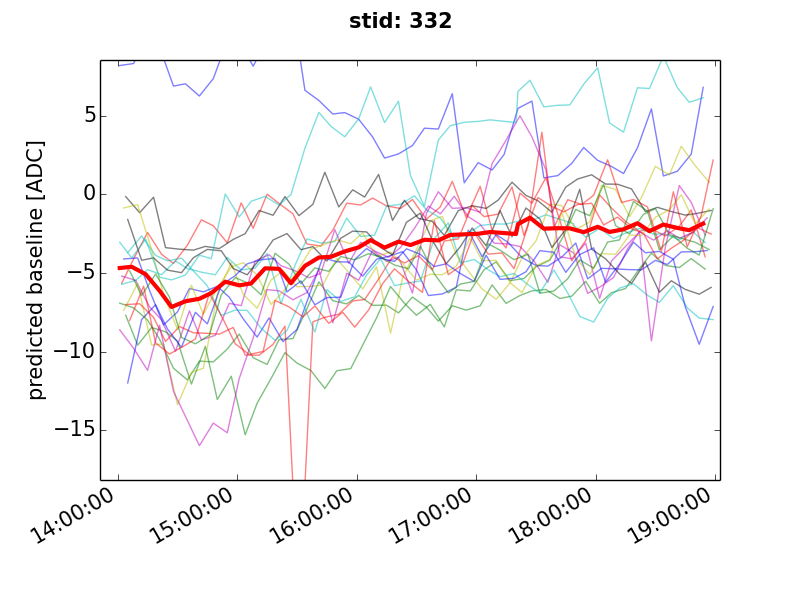
\includegraphics[width=0.32\linewidth]{yparam332.png}}
  \subfigure{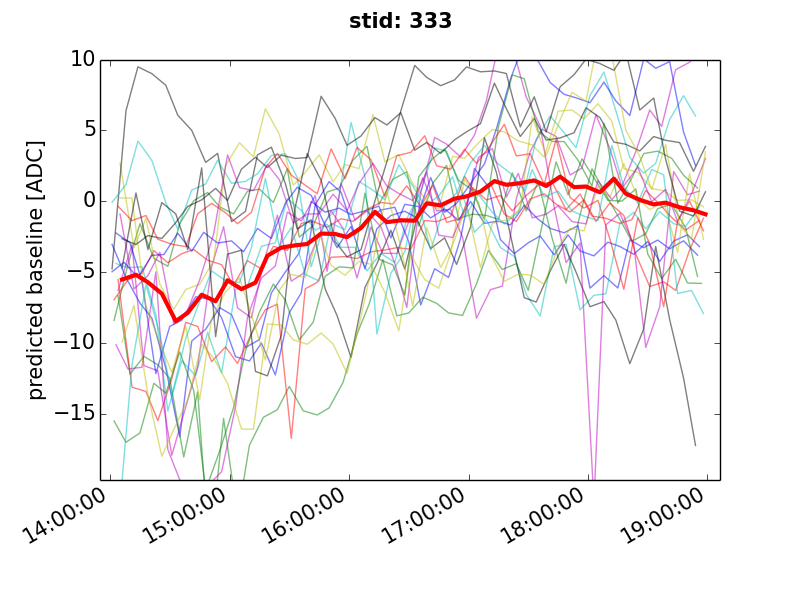
\includegraphics[width=0.32\linewidth]{yparam333.png}}
  \subfigure{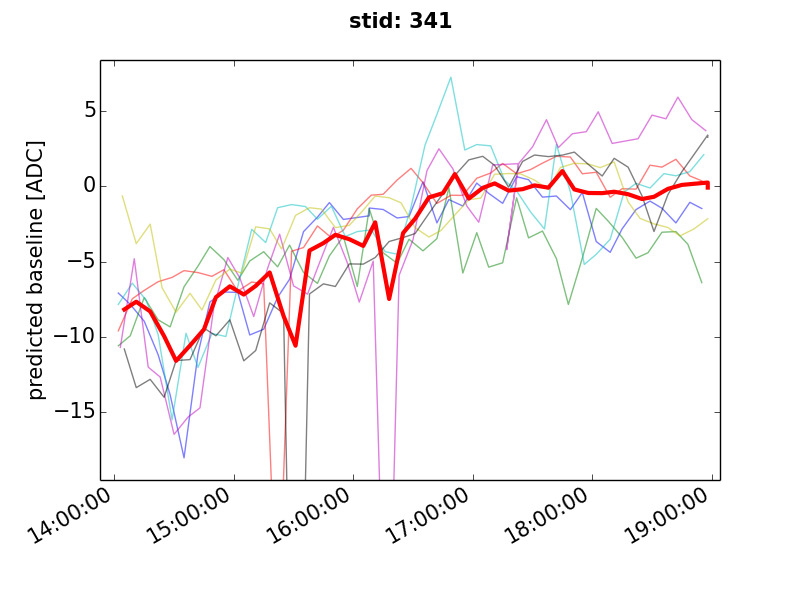
\includegraphics[width=0.32\linewidth]{yparam341.png}}\\
  \subfigure{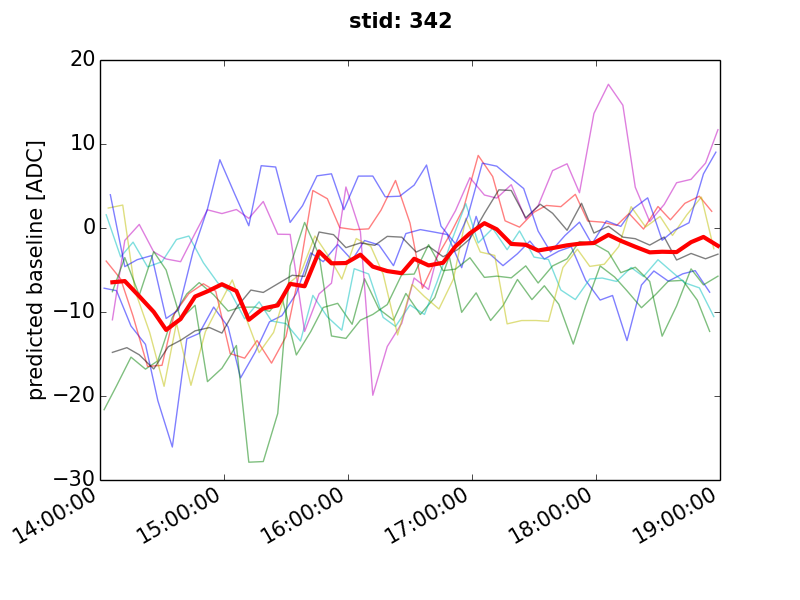
\includegraphics[width=0.32\linewidth]{yparam342.png}}
  \subfigure{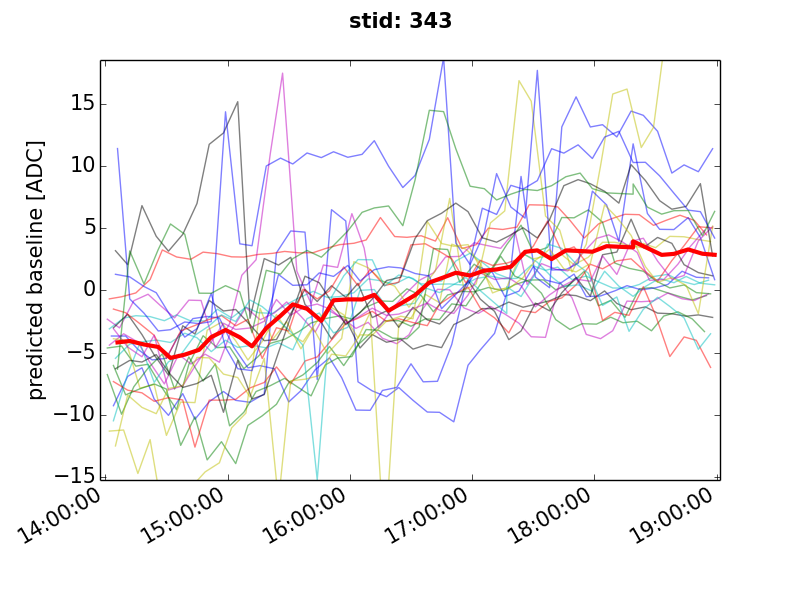
\includegraphics[width=0.32\linewidth]{yparam343.png}}
  \subfigure{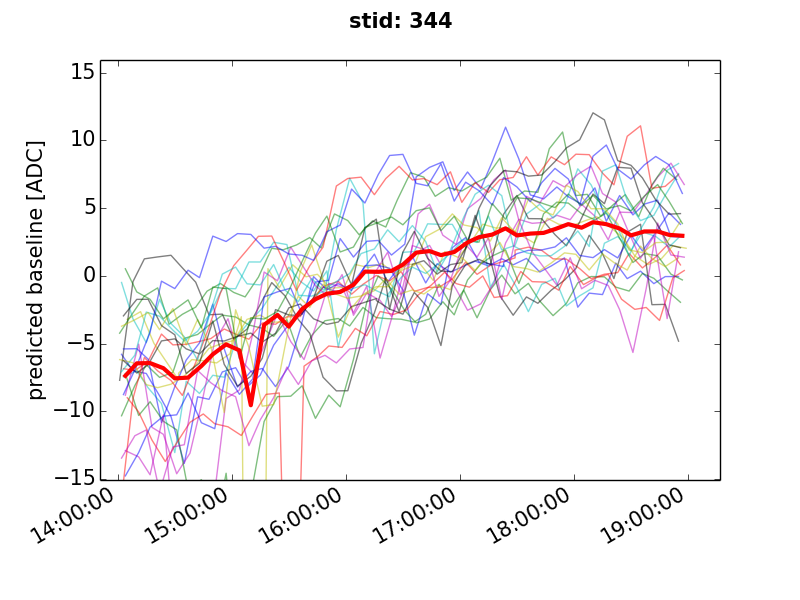
\includegraphics[width=0.32\linewidth]{yparam344.png}}
  \caption{baseline prediction with the temperature fit over a year}
  \label{fig:prediction1}
\end{figure}

\begin{figure}[!ht]
  \centering
  \hspace*{-3ex}
  \subfigure{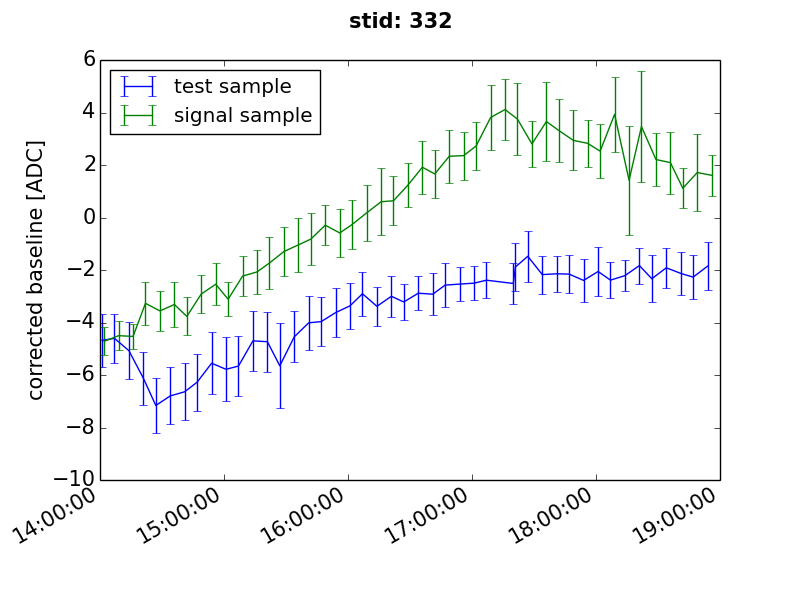
\includegraphics[width=0.32\linewidth]{yres332.png}}
  \subfigure{\includegraphics[width=0.32\linewidth]{yres333.png}}
  \subfigure{\includegraphics[width=0.32\linewidth]{yres341.png}}\\
  \subfigure{\includegraphics[width=0.32\linewidth]{yres342.png}}
  \subfigure{\includegraphics[width=0.32\linewidth]{yres343.png}}
  \subfigure{\includegraphics[width=0.32\linewidth]{yres344.png}}
  \caption{baseline prediction with the temperature fit over a year}
  \label{fig:prediction1}
\end{figure}

\newpage
\subsection{GIGADuck}
\begin{figure}[!ht]
  \centering
  \hspace*{-3ex}
  \subfigure{\includegraphics[width=0.9\linewidth]{GDnov.png}}
%%  \subfigure{\includegraphics[width=0.49\linewidth]{GDjanzoom.png}}
  \caption{}
  \label{fig:gigaduck}
\end{figure}

\begin{figure}[!ht]
  \centering
  \hspace*{-3ex}
  \subfigure{\includegraphics[width=0.9\linewidth]{GDblvstemp.png}}
%%  \subfigure{\includegraphics[width=0.49\linewidth]{GDjanzoom.png}}
  \caption{}
  \label{fig:gigaduck}
\end{figure}

%\include{signalfit/signalfit}
%\include{uncertainties/uncertainties}
%%\include{description/description}
%%\section*{conclusion}
We  have  gone  through  the  different step  to  simulate  an  EASIER
waveform.  In  particular, we  have detailed the  generation of  an RF
waveform from a realistic spectrum. We also improved the simulation of
the  adaptation  electronics. The  full  simulation  is then  compared
against  data looking at  the traces  fluctuation in  ADC.  We  find a
simulated waveform overestimated the  fluctuation by a small number of
ADC.


\addcontentsline{toc}{chapter}{Bibliography}                                 
\bibliographystyle{atlasnote}
\bibliography{thebib}
%% \newpage

\end{document}
